%=====================================================================
% Characteristic-frequency-guided spectral priors for bearing diagnosis
% IEEE conference format (IEEEtran). Compile with pdflatex (Overleaf: pdfLaTeX).
% Review-03 revision. Every number in the result tables is generated by
% scripts/make_review03_tables.py from outputs/review03/summary.json.
%=====================================================================
\documentclass[conference]{IEEEtran}
\IEEEoverridecommandlockouts
\usepackage{cite}
\usepackage{amsmath,amssymb,amsfonts}
\usepackage{algorithm}
\usepackage{algorithmic}
\usepackage[final]{graphicx}
\graphicspath{{figs/}{./}}
\setkeys{Gin}{draft=false}
\usepackage{textcomp}
\usepackage{xcolor}
\usepackage{booktabs}
\usepackage{array}
\usepackage{adjustbox} % shrink any table wider than its column
\usepackage{url}
\usepackage{listings}
\lstset{language=Python, basicstyle=\ttfamily\scriptsize,
  breaklines=true, breakatwhitespace=true, columns=fullflexible, keepspaces=true,
  frame=single, framerule=0.3pt, framesep=3pt, rulesep=0pt,
  xleftmargin=3pt, xrightmargin=3pt,
  aboveskip=8pt, belowskip=8pt, abovecaptionskip=3pt, belowcaptionskip=6pt,
  captionpos=t, numbers=none, showstringspaces=false,
  keywordstyle=\bfseries, commentstyle=\itshape\color{black!60}}
\def\BibTeX{{\rm B\kern-.05em{\sc i\kern-.025em b}\kern-.08em
    T\kern-.1667em\lower.7ex\hbox{E}\kern-.125emX}}
\newcommand{\Lspec}{L_{\mathrm{spec}}}

\begin{document}

\title{A Characteristic-Frequency-Constrained Physics-Informed\\
Neural Network (PINN) for Rolling-Element Bearing Fault Diagnosis\\
under Cross-Load Extrapolation on the CWRU Benchmark}

\author{\IEEEauthorblockN{Vaishvi Verma, Tanishq Garg, Sanchit Kumar,
and Kalyanaraman P\textsuperscript{*}}
\IEEEauthorblockA{\textit{School of Computer Science and Engineering} \\
\textit{Vellore Institute of Technology}, Vellore, India \\
\textsuperscript{*}Corresponding author: pkalyanaraman@vit.ac.in}
}

\maketitle

\begin{abstract}
Characteristic defect frequencies of rolling-element bearings follow in closed
form from the geometry and shaft speed, which makes them an appealing prior for
learned fault classifiers that must generalise across operating conditions. We
study a differentiable spectral-consistency term that rewards a predicted
fault type when the window's spectral energy lies at that type's defect
frequency and harmonics. We evaluate it on the original Case Western Reserve
University (CWRU) recordings and on the MFPT bearing data, with every split
formed before windowing so that overlapping windows cannot leak between
training and test. An audit of the term as first proposed shows three defects:
its 95\,Hz-resolution input cannot resolve the 68--490\,Hz defect harmonics
(physics-only fault-type accuracy 32\%, chance level), its differentiable
window weight pushes 64\% of faulty windows toward the healthy class, and its
mixture normalisation couples the gradient to mask mass. We derive a corrected
term on high-resolution raw or squared-envelope spectra whose gradient provably
leaves the healthy logit untouched. With five seeds and paired tests, an
identical CNN--LSTM without the prior reaches 99.3\,$\pm$\,1.0\% when trained at
0--2\,hp and tested on the unseen 3\,hp recordings, and 87.1\,$\pm$\,6.2\% when
trained at 0\,hp only. No variant of the prior improves on this significantly.
The envelope prior lowers 3\,hp accuracy to 97.6\% ($p=0.26$), and applying it
to unlabelled target windows lowers it to 89.6\% ($p<0.001$), because envelope
evidence alone identifies the fault type for only 66\% of real windows. Fixed
small weights are no worse than adaptive gradient-norm balancing, and the prior
gives no significant robustness gain under noise or emulated speed change. A
training-free sensitivity analysis shows that no band-width or harmonic setting
lifts the envelope evidence above 67\% on CWRU, whereas on the MFPT rig the same
evidence is 100\% correct and the unlabelled-target variant then classifies all
test windows correctly (preliminary, two seeds): the prior helps only where its
spectral evidence is reliable. We release CWRU-PG, a dataset derived from the
real CWRU recordings with leakage-free split labels, physics annotations and
stress-test variants, and report a component-wise ablation study. The
contribution is therefore an audited and corrected formulation evaluated under
leakage control, not an accuracy gain: the prior offers physical attributability
but does not improve diagnosis on CWRU. We position the method as a
physics-guided spectral prior rather than a differential-equation PINN and
release the full code and per-run results.
\end{abstract}

\begin{IEEEkeywords}
bearing fault diagnosis, physics-guided learning, characteristic frequency,
envelope analysis, domain shift, data leakage, CWRU, MFPT
\end{IEEEkeywords}

%=====================================================================
\section{Introduction}
%=====================================================================
Rolling-element bearings are among the most failure-prone components of
rotating machinery, and vibration-based condition monitoring is the standard
means of detecting their faults before a breakdown~\cite{jardine2006}. Deep
classifiers now report near-perfect accuracy on laboratory benchmarks such as
the Case Western Reserve University (CWRU) data~\cite{zhang2017,wen2018,hoang2019}.
Two questions are nevertheless left open by such figures: whether a
prediction can be related to a physical cause, and whether accuracy obtained
under one operating condition survives a change of condition that was never
seen in training~\cite{lei2020}. A third, more mundane question is whether the
figures are inflated by the evaluation itself: when overlapping windows of one
recording are scattered across training and test sets, test accuracy partly
measures memorisation of the recording~\cite{smith2015,zhao2020}.

A localized bearing defect produces a train of impacts whose repetition rate is
fixed by the bearing geometry and the shaft speed~\cite{mcfadden1984,randall2011}.
These characteristic defect frequencies are a natural source of prior knowledge
for a learned classifier. In an earlier version of this work we proposed a
spectral-consistency term that rewards a predicted fault class when the
window's spectral energy coincides with that class's defect frequency, and
assessed it on a dataset synthesised from the same frequency relations. The
present revision replaces that assessment with experiments on the original
recordings and re-examines the term itself. Our contributions are:

\begin{itemize}
\item An \emph{audit} of the spectral-consistency term as originally formulated.
We show, with measured quantities, that (i) its 95\,Hz-resolution STFT input
cannot resolve the 68--490\,Hz defect harmonics, so the prior is uninformative;
(ii) its probability-weighted normalisation lets the optimiser lower the
penalty by moving probability toward the healthy class; and (iii) the mixture
normalisation couples the gradient to the discretised mask mass of each class.
We give a corrected formulation (v2) with a high-resolution raw or
squared-envelope spectrum, equal-mass masks and a healthy-invariant,
stop-gradient window weight, and verify its gradient properties.
\item A precise positioning of the method as a \emph{physics-guided spectral
prior} rather than a differential-equation physics-informed neural network
(PINN): the term involves a kinematic relation and the observed spectrum, not
the residual of a governing equation.
\item A leakage-controlled evaluation on the original CWRU recordings
(in-distribution with time-blocked splits; 0/1/2$\to$3\,hp; 0$\to$3\,hp) with
five seeds, 95\% confidence intervals and paired tests, plus a preliminary
load-shift study on a second bearing dataset (MFPT). It isolates the physics term (identical CNN--LSTM with and without
it), compares fixed and adaptive weighting and raw and envelope spectra, and
tests robustness to noise and emulated speed change.
\item \emph{CWRU-PG}, a new dataset generated from the base CWRU recordings
with per-window provenance, leakage-free split labels, raw and envelope
spectra, physics annotations and noise/speed stress variants
(Section~\ref{sec:cwrupg}).
\item A component-wise ablation study of the physics term, its loss form,
spectral view, weighting, target-domain use and band settings
(Section~\ref{sec:ablation}).
\item Measured physics residuals: the departure of real CWRU signals from the
kinematic defect frequencies (frequency residual) and from the spectral prior
(spectral residual) (Section~\ref{sec:residuals}).
\item A training-free sensitivity analysis of the physical evidence over band
width and harmonic count on both datasets, which explains when the prior can
and cannot help.
\item Complete code and run files, so that every table entry can be regenerated
from the public recordings.
\end{itemize}

We report what the measurements show, including where the physics term does
not help.

%=====================================================================
\section{Related Work}
%=====================================================================
\subsection{Data-driven diagnosis on CWRU}
The CWRU Bearing Data Center recordings are the most widely used benchmark for
bearing diagnosis~\cite{cwru}. Smith and Randall's benchmark study with
envelope analysis found that most records are diagnosable but that several
ball-fault and some outer-race records do not show clear characteristic
signatures~\cite{smith2015}. Zhang \emph{et al.} proposed WDCNN, a wide-kernel
CNN on raw signals, and reported accuracy across motor loads, partly recovered
by adaptive batch normalisation~\cite{zhang2017}. Wen \emph{et al.} classified
signal images with a CNN~\cite{wen2018}, and Transformer encoders have also been
applied~\cite{costa2022}. Zhao \emph{et al.}'s open benchmark study warned that
splitting overlapping samples at random leaks test information into training
and inflates accuracy~\cite{zhao2020}; we therefore split along time before
segmentation.

\subsection{Bearing vibration physics}
McFadden and Smith modelled a point defect as an impulse train at the defect
frequency that excites structural resonances and is modulated by the load
distribution~\cite{mcfadden1984}. As a result, defect frequencies are often
invisible in the raw spectrum, which is dominated by resonances at several
kilohertz, but appear in the spectrum of the demodulated envelope. Randall and
Antoni's tutorial consolidates this envelope-analysis methodology~\cite{randall2011}.

\subsection{Physics-informed and physics-guided learning}
Physics-informed neural networks (PINNs) add the residual of a governing
differential equation, evaluated by automatic differentiation of the network
output at collocation points, to the training loss~\cite{raissi2019}; gradient
pathologies between data and residual terms motivate adaptive weighting
schemes~\cite{wang2021,mcclenny2023}. In fault diagnosis, physical knowledge
more often enters as features, architectural constraints or consistency
penalties than as an equation residual. Closest to our work, Alam \emph{et al.}
penalise a predicted inner- or outer-race fault that lacks envelope energy at
the corresponding characteristic frequency~\cite{alam2025}. We use a soft,
differentiable, per-window version of this idea and examine its optimisation
behaviour explicitly. Our held-out-load evaluation is a \emph{domain
generalisation} setting, in which no target-condition labels are available
during training; it therefore differs from domain-adaptation methods such as the
adaptive batch normalisation of~\cite{zhang2017}, which adapt to the target
distribution. The only variant that touches target-condition inputs is the
transductive one, which uses the \emph{unlabelled} 3\,hp (or 270--300\,lbs)
windows and is reported separately so that it is never conflated with the
label-free generalisation setting.

Table~\ref{tab:related} summarises the reviewed studies.

\begin{table*}[t]
\caption{Comparison of reviewed studies on bearing fault diagnosis and
physics-informed learning.}
\label{tab:related}
\centering
\footnotesize
\begin{adjustbox}{max width=\textwidth}
\begin{tabular}{p{2.5cm} p{2.4cm} p{3.2cm} p{4.0cm} p{3.2cm}}
\toprule
\textbf{Study} & \textbf{Dataset \& fault} & \textbf{Method} & \textbf{Key observation} & \textbf{Limitation / gap} \\
\midrule
Smith \& Randall (2015)~\cite{smith2015} & CWRU; all faults & Envelope-analysis benchmark & Most records diagnosable; some ball and outer-race records are not & Manual diagnosis; no learning model \\
Zhang \emph{et al.} (2017)~\cite{zhang2017} & CWRU; all faults & Wide-kernel CNN, AdaBN & High accuracy within a load; lower across loads & Purely data-driven \\
Wen \emph{et al.} (2018)~\cite{wen2018} & CWRU; all faults & Signal-to-image CNN & Near-ceiling in-distribution accuracy & In-distribution only \\
de Oliveira da Costa \emph{et al.} (2022)~\cite{costa2022} & CWRU, MaFaulDa & Transformer encoder & Near-ceiling in-distribution accuracy & No physical grounding \\
Zhao \emph{et al.} (2020)~\cite{zhao2020} & CWRU, MFPT, others & Open benchmark of deep models & Random window splits inflate accuracy & Benchmark; no physics prior \\
Alam \emph{et al.} (2025)~\cite{alam2025} & Paderborn, KAIST & 1D-CNN with characteristic-frequency penalty & Improved robustness under variable conditions & Thresholded trigger; not on CWRU cross-load \\
McFadden \& Smith (1984)~\cite{mcfadden1984} & Analytical model & Impact-train model & Explains defect signatures and modulation & Physical model only \\
Raissi \emph{et al.} (2019)~\cite{raissi2019} & Benchmark PDEs & PDE residual in the loss & Forward/inverse solution with sparse data & Requires a governing equation \\
\textbf{This work} & CWRU (4 classes), MFPT (3 classes) & Audited, corrected spectral prior; leakage-controlled protocols & See Section~\ref{sec:results} & Kinematic prior only; no dynamics \\
\bottomrule
\end{tabular}
\end{adjustbox}
\end{table*}

%=====================================================================
\section{Bearing Physics}
%=====================================================================
Let $f_r$ be the shaft rotation frequency and let the bearing have $n$ rolling
elements of diameter $d$ on a pitch diameter $D$ with contact angle $\phi$.
Under rolling without slip, a localized defect is struck at
\begin{align}
\mathrm{BPFO} &= \tfrac{n}{2}\, f_r \left(1 - \tfrac{d}{D}\cos\phi\right), \\
\mathrm{BPFI} &= \tfrac{n}{2}\, f_r \left(1 + \tfrac{d}{D}\cos\phi\right), \\
\mathrm{BSF}  &= \tfrac{D}{2d}\, f_r \left(1 - \left(\tfrac{d}{D}\cos\phi\right)^2\right), \\
\mathrm{FTF}  &= \tfrac{1}{2}\, f_r \left(1 - \tfrac{d}{D}\cos\phi\right),
\end{align}
for outer-race, inner-race, rolling-element and cage defects. Each frequency is
a geometry-fixed ratio $r_c$ times $f_r$, so the ratio does not depend on load,
although $f_r$ itself drops slightly with load (1797$\to$1730\,rpm on CWRU).
These relations are kinematic: they fix \emph{where} defect energy can appear,
but not \emph{how much} appears. Slip (measured on our data in
Section~\ref{sec:residuals}), resonance excitation,
load-zone modulation (inner-race and ball faults are amplitude-modulated at
$f_r$ and FTF respectively), and transmission-path effects are not described by
them~\cite{randall2011}. In the raw spectrum the defect frequencies are usually
buried beneath resonances at several kilohertz; demodulation (envelope
analysis) moves the impact repetition rate to baseband.
Fig.~\ref{fig:env} shows this on real CWRU windows: the raw spectrum carries
almost no energy at the defect harmonics, while the squared-envelope spectrum
peaks at BPFI and its harmonics for the inner-race fault and near BPFO for the
outer-race fault; the ball-fault window shows no clean BSF line, consistent
with~\cite{smith2015}.

\begin{figure*}[t]
\centering
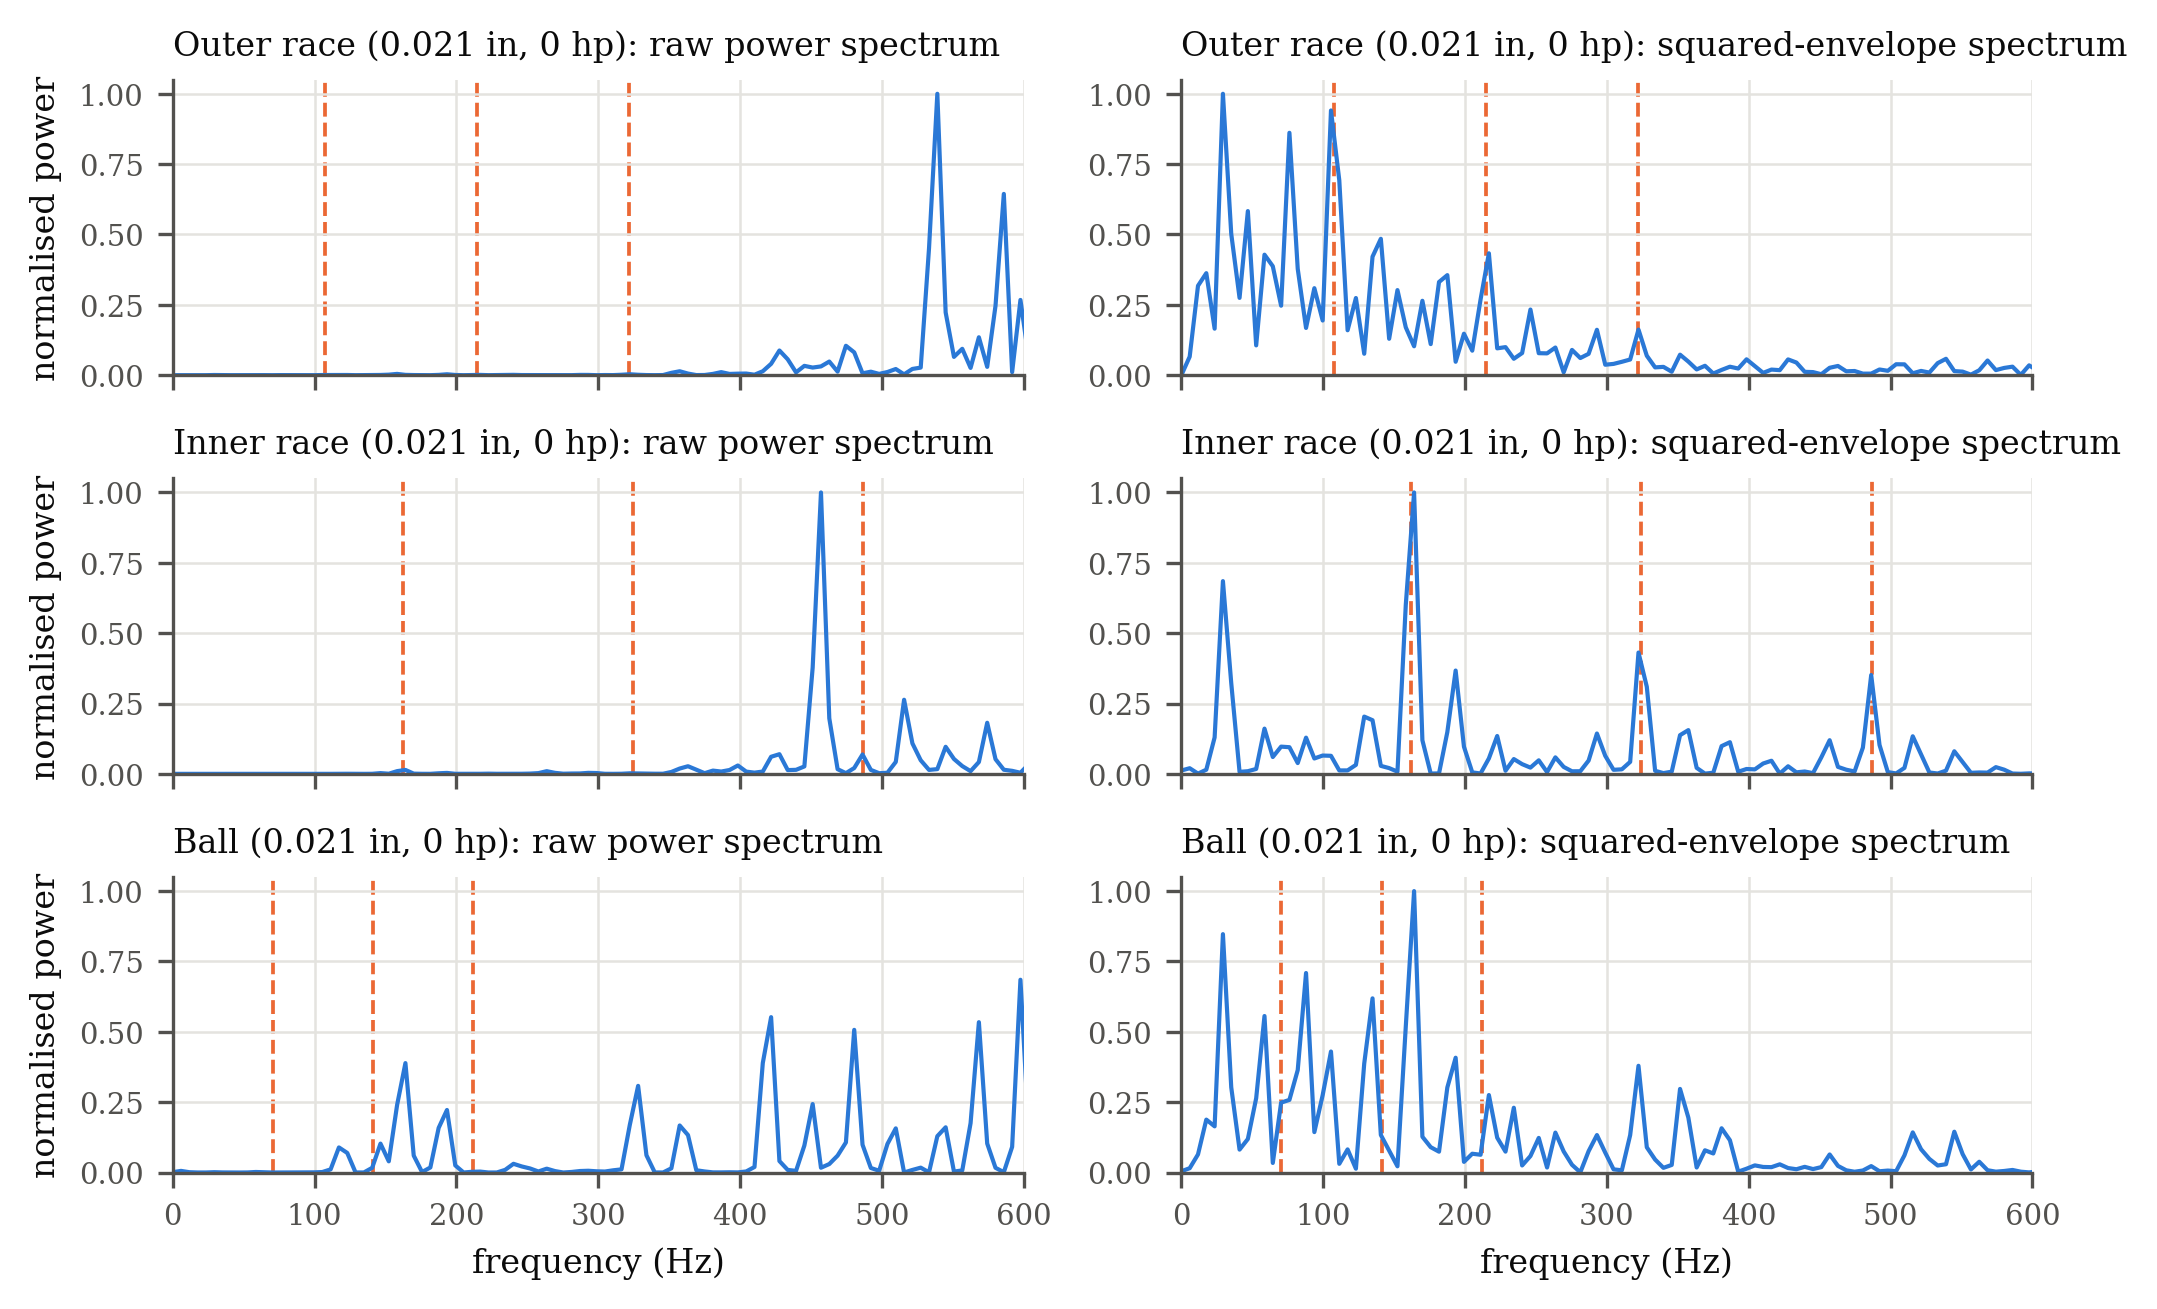
\includegraphics[width=0.92\textwidth]{fig_envelope_real.png}
\caption{Real CWRU drive-end windows (0\,hp, 0.021\,in faults; 2048 samples at
12\,kHz). Left: raw power spectrum. Right: squared-envelope spectrum
(1--5.5\,kHz band). Dashed lines: first three harmonics of the class's
characteristic frequency computed from the recorded shaft speed.}
\label{fig:env}
\end{figure*}

%=====================================================================
\section{Data and Leakage-Controlled Protocols}
\label{sec:data}
%=====================================================================
\subsection{CWRU recordings}
We use 40 original drive-end recordings at 12\,kHz from the CWRU Bearing Data
Center~\cite{cwru} (SKF-6205; Table~\ref{tab:params}): the four normal baseline
recordings (files 97--100) and inner-race, ball and outer-race (centred, 6:00)
faults of 0.007, 0.014 and 0.021\,in at motor loads 0--3\,hp (files 105--108,
118--121, 130--133, 169--172, 185--188, 197--200, 209--212, 222--225,
234--237). The normal baselines were acquired at 48\,kHz~\cite{smith2015} and
are decimated by four with an anti-aliasing polyphase filter. Each fault
recording lasts about 10\,s. The shaft speed stored with each file is used to
compute its characteristic frequencies. The task is four-class
(healthy/inner/outer/ball), with all three severities pooled per class.

\begin{table}[t]
\caption{Bearing parameters and characteristic-frequency ratios.}
\label{tab:params}
\centering
\footnotesize
\begin{adjustbox}{max width=\columnwidth}
\begin{tabular}{lcc}
\toprule
Parameter & CWRU (SKF-6205) & MFPT (NICE) \\
\midrule
Rolling elements $n$ & 9 & 8 \\
Element diameter $d$ (in) & 0.3126 & 0.235 \\
Pitch diameter $D$ (in) & 1.537 & 1.245 \\
Contact angle $\phi$ & $0^{\circ}$ & $0^{\circ}$ \\
Shaft frequency $f_r$ (Hz) & 28.7--29.9 (recorded) & 25 \\
$\mathrm{BPFO}/f_r$ & 3.585 & 3.245 \\
$\mathrm{BPFI}/f_r$ & 5.415 & 4.755 \\
$\mathrm{BSF}/f_r$ & 2.357 & 2.555 \\
$\mathrm{FTF}/f_r$ & 0.398 & 0.406 \\
\bottomrule
\end{tabular}
\end{adjustbox}
\end{table}

\subsection{MFPT recordings}
As a second dataset we use the MFPT bearing data~\cite{mfpt} (NICE bearing, 25\,Hz shaft):
the 270\,lbs healthy baseline, the 270\,lbs outer-race record, and inner- and
outer-race records at four of the seven variable loads (inner: 0, 50, 150,
300\,lbs; outer: 25, 50, 150, 300\,lbs). The MFPT website no longer hosts the
files; we used a public mirror whose checksum is recorded in the code
repository. All records are decimated to 12.2\,kHz so that a 2048-sample window
spans a similar time as on CWRU. The task is three-class (no ball fault).

\subsection{Splitting before windowing}
Windows are 2048 samples with 50\% overlap. To avoid leakage, every split is
formed on the continuous recordings \emph{before} any window is cut:
\begin{itemize}
\item \emph{In-distribution (CWRU):} each recording is cut into three
contiguous time blocks (70/15/15\%) separated by a guard gap of one window
length; windows are then cut within each block.
\item \emph{Cross-load 0/1/2$\to$3\,hp (CWRU):} the ten 3\,hp recordings
(one healthy, nine faulty) form the test set as whole recordings; each 0--2\,hp recording is time-blocked
85/15\% into training and validation.
\item \emph{Single-source 0$\to$3\,hp (CWRU):} as above, training on 0\,hp
recordings only.
\item \emph{Load shift (MFPT):} fault records at 0--150\,lbs train/validate
(85/15\% time blocks); the 270 and 300\,lbs fault records are the test set.
Healthy data exist only at 270\,lbs and are time-blocked 70/15/15\%.
\end{itemize}
After windowing, an automated check confirms that no two windows in different
splits share a sample. Feature standardisation statistics come from the
training windows only. Table~\ref{tab:protocols} lists the resulting sizes.
Because the CWRU set has a single recording per class, severity and load, a
split by recording within one load is impossible without removing a whole
fault condition from training; the time-blocked in-distribution split is the
leakage-free alternative, and the cross-load protocols are split by recording.

% --- generated by scripts/make_review03_tables.py (tables/tab_protocols.tex) ---
\begin{table}[t]
\caption{Leakage-controlled protocols: windows (recordings) per split. Splits are formed before windowing; no two windows in different splits share a sample.}
\label{tab:protocols}
\centering
\footnotesize
\begin{adjustbox}{max width=\columnwidth}
\begin{tabular}{llccc}
\toprule
Protocol & Split & Windows & Recordings & Loads \\
\midrule
CWRU in-dist. & train & 3118 & 40 & 0,1,2,3 \\
 & val & 631 & 40 & 0,1,2,3 \\
 & test & 631 & 40 & 0,1,2,3 \\
\midrule
CWRU 0/1/2$\to$3 hp & train & 2887 & 30 & 0,1,2 \\
 & val & 471 & 30 & 0,1,2 \\
 & test & 1178 & 10 & 3 \\
\midrule
CWRU 0$\to$3 hp & train & 929 & 10 & 0 \\
 & val & 151 & 10 & 0 \\
 & test & 1178 & 10 & 3 \\
\midrule
MFPT load shift & train & 208 & 7 & 0,25,50,150,270 \\
 & val & 33 & 7 & 0,25,50,150,270 \\
 & test & 147 & 4 & 270,300 \\
\bottomrule
\end{tabular}
\end{adjustbox}
\end{table}


\subsection{Relation to the earlier constructed dataset}
The previous version evaluated the method on 1{,}536 windows synthesised by
placing impact trains at the theoretical defect frequencies. Because the
physics term rewards exactly those frequencies, success on that data
demonstrated compatibility with the assumed model rather than robustness to
unmodelled phenomena such as slip, resonance excitation, modulation, noise and
transmission paths. The constructed data are not used for any result in this
paper. The only results retained from the earlier version are analytical checks
that the physics module reproduces the closed-form ratios (Table~\ref{tab:freq}).

\subsection{CWRU-PG: a physics-guided dataset derived from CWRU}
\label{sec:cwrupg}
Building on the base CWRU benchmark and on the envelope-analysis studies
reviewed in Section~II~\cite{smith2015,randall2011}, we generate a new dataset,
\emph{CWRU-PG} (physics-guided), from the 40 original recordings. Unlike the
earlier constructed dataset, CWRU-PG contains no synthesised signals: every
window is cut from a real recording, and every physical quantity attached to
it is computed from the measured signal and the recorded shaft speed. The
generation pipeline has five steps.
\begin{enumerate}
\item \emph{Windowing with provenance.} Each recording is cut into 2048-sample
windows with 50\% overlap. Each window keeps its recording identifier, start
sample, class, fault diameter, motor load and recorded shaft speed.
\item \emph{Leakage-free split labels.} For each protocol of
Section~\ref{sec:data} (in-distribution time blocks, 0/1/2$\to$3\,hp,
0$\to$3\,hp), every window is labelled \emph{train}, \emph{val}, \emph{test} or
\emph{unused}. Windows falling in a guard gap are marked unused, so any
user of the dataset inherits the leakage-free splits.
\item \emph{Learning inputs.} Each window has a $64\times64$ STFT map, four
waveform statistics and twelve handcrafted features.
\item \emph{Physics views and annotations.} Each window also stores:
\begin{itemize}
\item the raw and squared-envelope power spectra (0--1\,kHz, 5.9\,Hz bins);
\item its own BPFO, BPFI and BSF;
\item the per-fault-type evidence $\bar e_{bc}$ of Eq.~\eqref{eq:v2};
\item the evidence-only fault-type prediction.
\end{itemize}
\item \emph{Stress-test variants.} The ten 3\,hp recordings are re-generated
under additive white noise (10, 5, 0, $-5$\,dB) and emulated speed change
($\times0.95$, $\times1.05$, $\pm5\%$ fluctuation). The same features, spectra
and annotations are stored for each variant.
\end{enumerate}

Table~\ref{tab:cwrupg} summarises the dataset. It contains 4{,}643 real windows
plus 8{,}187 stress-test windows. The physics annotations make the limits of
the kinematic prior visible at dataset level:
\begin{itemize}
\item \emph{Overall:} envelope evidence alone identifies the fault type of
66.0\% of the faulty windows.
\item \emph{By fault type:} inner race 74.4\%, outer race 72.7\%, ball 50.8\%.
\item \emph{By severity:} 82.7\% for 0.007\,in faults, but only 48.3\% for
0.014\,in faults.
\item \emph{By load:} it falls slightly with load, from 68.8\% at 0\,hp to
64.1\% at 3\,hp.
\item \emph{Under stress:} it degrades to 58.1\% at $-5$\,dB and 57.8\% under
speed fluctuation.
\end{itemize}
The dataset is released as compressed NumPy archives with a per-window CSV
index and a datasheet. Raw windows are not duplicated: they are regenerated
from the public CWRU files and the stored start indices.

\begin{table}[t]
\caption{Composition of the derived CWRU-PG dataset and the measured accuracy
of its physics annotations (fault windows; envelope evidence, $\sigma=5$\,Hz,
$H=3$).}
\label{tab:cwrupg}
\centering
\footnotesize
\begin{adjustbox}{max width=\columnwidth}
\begin{tabular}{llc}
\toprule
Group & Subset & Value \\
\midrule
Windows (real) & healthy / inner / outer / ball & 409 / 1410 / 1413 / 1411 \\
 & 0 / 1 / 2 / 3\,hp & 1116 / 1175 / 1174 / 1178 \\
Stress variants & 7 variants of the 3\,hp recordings & 8187 windows \\
\midrule
Evidence acc.\ (\%) & all fault windows & 66.0 \\
 & inner / outer / ball & 74.4 / 72.7 / 50.8 \\
 & 0.007 / 0.014 / 0.021\,in & 82.7 / 48.3 / 66.8 \\
 & 0 / 1 / 2 / 3\,hp & 68.8 / 66.5 / 64.4 / 64.1 \\
 & noise 10 / 5 / 0 / $-5$\,dB & 62.8 / 61.7 / 60.6 / 58.1 \\
 & speed $\times0.95$ / $\times1.05$ / $\pm5\%$ & 61.6 / 64.3 / 57.8 \\
\bottomrule
\end{tabular}
\end{adjustbox}
\end{table}

\subsection{Constraint values and limits derived from CWRU-PG}
\label{sec:limits}
CWRU-PG also gives the numerical constraint values used by the prior and
practical limits for diagnosis (Table~\ref{tab:limits}); no model is trained
for any of them.
\begin{itemize}
\item \emph{Physics constraint values.} Over the recorded shaft speeds
(28.7--30.0\,Hz), the defect frequencies the prior enforces lie at
102.8--107.4\,Hz (BPFO), 155.3--162.2\,Hz (BPFI) and 67.6--70.6\,Hz (BSF).
\item \emph{Per-class ranges.} The table reports the median and the
5th--95th percentile range of RMS, excess kurtosis and crest factor for each
class.
\item \emph{Alarm limits.} For each statistic, the healthy-versus-faulty limit
is chosen on the 0--2\,hp training windows and checked on the unseen 3\,hp
windows. RMS is by far the most reliable: above 0.082 it detects 99.6\% of
faulty 3\,hp windows with no false alarm. Kurtosis and crest-factor limits
detect only 69--72\% of faults, with 10\% false alarms.
\item \emph{Reliability limit of the physics prior.} Let the evidence margin
be the gap between the strongest and the second-strongest fault evidence.
\begin{itemize}
\item On the unseen 3\,hp windows, the evidence label is 93.9\% correct when
the margin is at least 0.49 (39\% of fault windows).
\item It is 89.0\% correct at a margin of at least 0.40 (44\% of fault
windows).
\item Below these thresholds it is right only 44--45\% of the time.
\end{itemize}
This threshold marks where the kinematic constraint can be trusted.
\end{itemize}
The alarm limits are specific to this rig, sensor and data scaling, and the
healthy class contains only four recordings (one per load), so the false-alarm
rates rest on a single 3\,hp healthy recording.

\begin{table}[t]
\caption{Constraint values and limits derived from CWRU-PG (measured). Class
ranges: median [5th, 95th percentile]. Alarm limits and evidence thresholds
are chosen on the 0--2\,hp training windows and evaluated on the unseen 3\,hp
windows.}
\label{tab:limits}
\centering
\footnotesize
\begin{adjustbox}{max width=\columnwidth}
\begin{tabular}{lll}
\toprule
Group & Quantity & Value \\
\midrule
Physics constraints & Shaft frequency $f_r$ & 28.7--30.0\,Hz \\
 & BPFO / BPFI / BSF & 102.8--107.4 / 155.3--162.2 / 67.6--70.6\,Hz \\
\midrule
RMS & healthy / inner & 0.059 [0.056, 0.072] / 0.296 [0.158, 0.521] \\
 & outer / ball & 0.559 [0.091, 0.668] / 0.135 [0.100, 0.186] \\
Excess kurtosis & healthy / inner & $-0.03$ [$-0.26$, 0.17] / 4.7 [2.2, 20.8] \\
 & outer / ball & 4.8 [$-0.14$, 21.8] / 0.30 [$-0.24$, 8.1] \\
Crest factor & healthy / inner & 3.57 [3.15, 4.17] / 5.83 [4.39, 9.72] \\
 & outer / ball & 4.99 [3.30, 9.62] / 3.93 [3.17, 7.86] \\
\midrule
Alarm limit (3\,hp) & RMS $>0.082$ & detect 99.6\%, false alarm 0.0\% \\
 & Kurtosis $>0.20$ & detect 72.0\%, false alarm 10.3\% \\
 & Crest factor $>4.15$ & detect 69.0\%, false alarm 10.3\% \\
\midrule
Evidence reliability & margin $\ge0.40$ & 89.0\% correct, covers 44.5\% \\
(3\,hp, fault windows) & margin $\ge0.49$ & 93.9\% correct, covers 38.9\% \\
 & below threshold & 44.1--45.1\% correct \\
\bottomrule
\end{tabular}
\end{adjustbox}
\end{table}

\subsection{Physics residuals}
\label{sec:residuals}
In a PINN the residual $r=\mathcal N[u]$ measures how far a quantity departs
from the governing equation. For the kinematic relations of Section~III, the
natural residuals measure how far the real signals depart from the assumed
physics. We report two of them, computed without training
(Table~\ref{tab:residuals}).

\textbf{Frequency residual.} For every fault recording we compute
$r_f=f_{\mathrm{obs}}-f_{\mathrm{th}}$, where $f_{\mathrm{th}}$ is the
theoretical BPFI, BPFO or BSF at the recorded shaft speed. The observed line
$f_{\mathrm{obs}}$ is the strongest squared-envelope peak within $\pm5\%$ of
$f_{\mathrm{th}}$, computed over the whole $\approx$10\,s recording
($\approx$0.1\,Hz resolution, parabolic peak interpolation). A line counts as
present when its prominence (peak over median power in the search band)
exceeds 10.
\begin{itemize}
\item \emph{Inner race:} lines are present in all 12 recordings and lie
$-0.29\pm0.15$\,Hz ($-0.18\%$) below BPFI.
\item \emph{Outer race:} lines are present in 11 of 12 recordings, at
$+0.36\pm0.21$\,Hz ($+0.34\%$) above BPFO.
\item \emph{Ball:} a line is present in only 6 of 12 recordings. Where
present, it sits consistently $+1.32\pm0.09$\,Hz ($+1.8$ to $+2.1\%$) above
BSF.
\end{itemize}
All residuals of the present lines are well inside the $\sigma=5$\,Hz masks,
so a misplaced line is not the main failure mode. The prior fails mainly where
the line is \emph{absent}. Notably, none of the four 0.014\,in ball recordings
shows a ball-spin line, which matches the low evidence accuracy at that
severity (48.3\%, Table~\ref{tab:cwrupg}). The small, stable race residuals
confirm that, when present, the kinematic frequencies are accurate to better
than 1\%.

\textbf{Spectral (consistency) residual.} Per window we define
$r_s=1-\bar e_{b,y}$: the shortfall of the true fault type's evidence relative
to the strongest fault evidence. It is the per-window value that
$\Lspec^{\mathrm{v2}}$ penalises when the network predicts the true class.
\begin{itemize}
\item $r_s=0$ for 66.0\% of fault windows.
\item Its mean is 0.098 and its 90th percentile 0.40.
\item It is largest for ball faults (mean 0.165) and rises slightly with load
(0.088 at 0\,hp to 0.106 at 3\,hp).
\end{itemize}
A non-zero $r_s$ on a correctly labelled window is exactly the case in which
the prior pushes the network toward a wrong fault type.

\begin{table}[t]
\caption{Physics residuals on the real CWRU data (measured, no training).
Frequency residual $r_f=f_{\mathrm{obs}}-f_{\mathrm{th}}$ per recording (mean
$\pm$ s.d.\ over recordings with a present line); spectral residual
$r_s=1-\bar e_{b,y}$ per window.}
\label{tab:residuals}
\centering
\footnotesize
\begin{adjustbox}{max width=\columnwidth}
\begin{tabular}{lccc}
\toprule
Frequency residual & Inner (BPFI) & Outer (BPFO) & Ball (BSF) \\
\midrule
Line present (recordings) & 12/12 & 11/12 & 6/12 \\
\quad by 0.007 / 0.014 / 0.021\,in & 4 / 4 / 4 & 4 / 3 / 4 & 4 / 0 / 2 \\
$r_f$ (Hz) & $-0.29\pm0.15$ & $+0.36\pm0.21$ & $+1.32\pm0.09$ \\
$r_f$ (\% of $f_{\mathrm{th}}$) & $-0.18\pm0.10$ & $+0.34\pm0.20$ & $+1.91\pm0.13$ \\
\midrule
Spectral residual $r_s$ & Inner & Outer & Ball \\
\midrule
Mean / 90th percentile & 0.060 / 0.28 & 0.069 / 0.32 & 0.165 / 0.50 \\
Fraction with $r_s=0$ & 74.4\% & 72.7\% & 50.8\% \\
\midrule
$r_s$ mean by load (0/1/2/3\,hp) & \multicolumn{3}{c}{0.088 / 0.093 / 0.104 / 0.106} \\
\bottomrule
\end{tabular}
\end{adjustbox}
\end{table}

%=====================================================================
\section{Method}
\label{sec:method}
%=====================================================================
\subsection{Network and inputs}
Each window is mapped to a $64\times64$ log-magnitude STFT image (0--6\,kHz,
min--max normalised) and to four waveform statistics (RMS, kurtosis, crest
factor, skewness). Three convolutional blocks (16, 32, 64 filters, $3\times3$,
batch normalisation, ReLU, max-pooling) are followed by a two-layer LSTM (128
units), fusion with the statistics into a 128-dimensional embedding (dropout
0.3), and a classification head (2.35\,M parameters). Every physics variant
uses exactly this network; the baseline is the same network with $\lambda=0$.
The physics term enters only the training loss: at inference the model sees
the same inputs as the baseline and needs no shaft-speed measurement.

\subsection{Spectral-consistency term as originally formulated (v1)}
Let $\mathbf{p}_b$ be the softmax output for window $b$, $\mathcal{K}$ the
set of fault classes, and $m_{bc}(f)=\sum_{h=1}^{H}\exp(-(f-h r_c f_{r,b})^2/2\sigma^2)$,
scaled to unit maximum, with $m_{bc}\equiv0$ for the healthy class. The earlier
version used
\begin{equation}
\begin{aligned}
\Lspec^{\mathrm{v1}} &= \frac{\sum_b w_b\,\bigl(1-\sum_f s_{bf}\,\hat m_{bf}\bigr)}{\sum_b w_b},\\
\hat m_b &= \frac{\sum_c p_{bc}\, m_{bc}}{\sum_{f,c} p_{bc}\, m_{bcf}},\qquad
w_b=\sum_{c\in\mathcal K}p_{bc},
\end{aligned}
\label{eq:v1}
\end{equation}
with $s_b$ the time-summed $64\times64$ STFT image normalised to unit sum.

\textbf{Audit.} We checked the normalisation, the healthy zero mask and the
gradient flow of~\eqref{eq:v1} on the real training windows
(Table~\ref{tab:audit}).
\begin{enumerate}
\item \emph{Resolution.} The STFT rows are 95\,Hz apart, so all defect
harmonics up to $3\times$BPFI (487\,Hz) fall in the lowest six rows, and the
log compression flattens their differences. Used as a classifier on its own,
the prior identifies the fault type of 32\% of fault windows, which is chance level
for three types. With $s$ independent of the network parameters, its gradient is
also tiny ($\sim10^{-6}$ per logit), which drives the adaptive weight to
large values.
\item \emph{Healthy shortcut.} Since $w_b$ is differentiable,
$\partial\Lspec^{\mathrm{v1}}/\partial w_b=(\ell_b-\Lspec^{\mathrm{v1}})/\sum_b w_b$.
Windows whose spectrum aligns worse than the batch average are therefore
pushed toward \emph{lower} fault probability, i.e.\ toward ``healthy'',
regardless of their label: this happens for 64\% of the faulty training
windows. The zero healthy mask thus does not make the term neutral to the
healthy class.
\item \emph{Mask-mass coupling.} Normalising the probability-weighted mixture
makes the alignment a weighted mean of per-class alignments with weights
$p_{bc}\lVert m_{bc}\rVert_1$, so classes whose discretised mask has more mass
(here inner/outer 3.2 vs.\ ball 2.3) receive more pull.
\end{enumerate}

% --- generated by scripts/make_review03_tables.py (tables/tab_audit.tex) ---
\begin{table}[t]
\caption{Audit of the spectral-consistency term on the CWRU 0--2\,hp training windows (measured, no training involved).}
\label{tab:audit}
\centering
\footnotesize
\begin{adjustbox}{max width=\columnwidth}
\begin{tabular}{lccc}
\toprule
Quantity & v1 (STFT) & Raw & Envelope \\
\midrule
Bin width (Hz) & 95.2 & 5.9 & 5.9 \\
Physics-only fault-type acc.\ (\%) & 32.3 & 33.3 & 66.4 \\
\quad inner recall (\%) & 88.9 & 100.0 & 74.5 \\
\quad outer recall (\%) & 8.0 & 0.0 & 74.5 \\
\quad ball recall (\%) & 0.0 & 0.0 & 50.3 \\
\midrule
\multicolumn{4}{l}{\emph{Gradient of the loss w.r.t.\ logits (random logits, 512 windows)}} \\
Mean $|\partial L/\partial z_{\mathrm{healthy}}|$ & 1.9e-06 & \multicolumn{2}{c}{v2: 0.0 (exact)} \\
Mean $|\partial L/\partial z_{\mathrm{fault}}|$ & 1.2e-06 & \multicolumn{2}{c}{v2: 1.1e-04} \\
Faulty windows pushed toward healthy (\%) & 63.5 & \multicolumn{2}{c}{v2: 0.0} \\
True fault logit raised by descent (\%) & -- & \multicolumn{2}{c}{v2 (envelope): 76.0} \\
\bottomrule
\end{tabular}
\end{adjustbox}
\end{table}


\subsection{Revised term (v2)}
We change the representation and the normalisation. The spectrum $s_b$ is now
computed from the window itself with a 2048-point Hann FFT (5.9\,Hz bins,
0--1\,kHz), either the raw power spectrum or the squared-envelope spectrum
$|\mathcal F\{|\mathcal H\{x_{\mathrm{bp}}\}|^2-\mu\}|^2$ of the 1--5.5\,kHz
band-passed signal~\cite{randall2011}. Masks are scaled to unit \emph{sum}, so
every fault class has the same mass. With per-window evidence
$e_{bc}=\sum_f s_{bf} m_{bcf}$ and its rescaling
$\bar e_{bc}=e_{bc}/\max_{c'}e_{bc'}\in[0,1]$,
\begin{equation}
\Lspec^{\mathrm{v2}}=\frac{\sum_b \bar w_b\,\bigl(1-\sum_{c\in\mathcal K}\tilde p_{bc}\,\bar e_{bc}\bigr)}{\sum_b \bar w_b},
\label{eq:v2}
\end{equation}
where $\tilde p_{bc}=\exp z_{bc}/\sum_{c'\in\mathcal K}\exp z_{bc'}$ is the
fault-type distribution from the fault logits only, and
$\bar w_b=\mathrm{sg}(\sum_{c\in\mathcal K}p_{bc})$ is a stop-gradient window
weight. Consequently $\partial\Lspec^{\mathrm{v2}}/\partial z_{\mathrm{healthy}}=0$
exactly: the term never moves probability into or out of the healthy class,
and among fault types it moves probability toward the type with the stronger
evidence. Unit tests verify both properties.
Healthy windows contribute little because $\bar w_b$ is small once the network
recognises them, while the cross-entropy alone decides healthy versus faulty.

\subsection{Physics-guided prior versus differential-equation PINN}
\label{sec:notpinn}
Equation~\eqref{eq:v2} is not a PINN residual in the sense of~\cite{raissi2019}.
A PINN penalises $\mathcal N[u_\theta]=0$ for a governing operator $\mathcal N$
applied to the network output $u_\theta$, at collocation points where no labels
are needed, so the physics supplies a constraint independent of the
measurements. Here no dynamical equation is solved or enforced: the term
combines a kinematic relation ($f_c=r_c f_r$) with the \emph{observed} spectrum
of the same input the network sees, and acts as a spectral pseudo-label for the
fault type. It therefore encodes neither resonance dynamics nor slip or
modulation, and it can only be as good as the spectral evidence. We refer to
it as a physics-\emph{guided} spectral prior. Accordingly, the residuals we
report (Section~\ref{sec:residuals}) measure the data's departure from the
kinematic relations, not the violation of a differential equation by the
network. The closest analogue to PINN
collocation is to apply the term on unlabelled windows of the target
condition; we evaluate this variant separately and mark it as transductive,
because it uses test-condition inputs (never their labels).

\subsection{Relation to conventional frequency-domain preprocessing}
\label{sec:novelty}
Characteristic defect frequencies and envelope analysis are long-established
descriptors~\cite{mcfadden1984,randall2011}, so the contribution here is not the
descriptor but its use and its scrutiny. The relation is embedded as a soft,
differentiable constraint on the shared representation during training, rather
than as a precomputed feature or a post-hoc peak test, so it can in principle
shape what the network learns instead of only labelling its input. We then
\emph{isolate} that influence: every physics run is compared against an
identical network that sees the same inputs but carries no constraint, which
measures whatever the term contributes \emph{beyond} what the data-driven
classifier already extracts from the same spectrum. This isolation is the
mechanism that lets us answer the novelty question quantitatively rather than by
assertion. On CWRU the measured answer is that the constraint adds nothing: the
envelope evidence it encodes is already available to, and better exploited by,
the unconstrained classifier (Section~\ref{sec:results}). We therefore report
the isolation and its outcome, not a claim that the descriptor itself is new.

\subsection{Weighting}
The training loss is $L=L_{\mathrm{CE}}+\lambda\Lspec$ with class-weighted
cross-entropy. We compare fixed $\lambda\in\{0.1,0.5,1.0\}$ with an adaptive
rule that, at every step, sets the target
$\hat\lambda=\rho\,\lVert\nabla_\theta L_{\mathrm{CE}}\rVert/\lVert\nabla_\theta\Lspec\rVert$
over the shared backbone parameters, with $\rho=0.25$, and tracks it with an
exponential moving average ($\alpha=0.12$), in the spirit
of~\cite{wang2021,mcclenny2023}. Algorithm~\ref{alg:train} summarises one step.

\begin{algorithm}[t]
\caption{Training step with the revised spectral prior}
\label{alg:train}
\begin{algorithmic}[1]
\STATE \textbf{Input:} STFT images $X$, statistics $Z$, labels $y$, spectra $S$ (raw or envelope), shaft speeds $f_r$
\STATE $z \leftarrow \mathrm{model}(X,Z)$;\ $L_{\mathrm{CE}}\leftarrow\mathrm{CE}_{\mathrm{w}}(z,y)$
\STATE masks $m_{bc}$ from $h\,r_c f_{r,b}$, $h=1..H$, unit sum
\STATE $\bar e\leftarrow$ evidence of $S$ under $m$; $\tilde p\leftarrow$ softmax over fault logits
\STATE $\Lspec\leftarrow$ Eq.~\eqref{eq:v2} with stop-gradient weights
\STATE (transductive variant: add Eq.~\eqref{eq:v2} on an unlabelled target batch)
\STATE if adaptive: update $\lambda$ from the gradient-norm ratio
\STATE back-propagate $L_{\mathrm{CE}}+\lambda\Lspec$; clip gradients at 5; Adam step
\end{algorithmic}
\end{algorithm}

%=====================================================================
\section{Experimental Setup}
%=====================================================================
\textbf{Models.} Random forest (300 trees) and RBF-SVM ($C=10$) on twelve
handcrafted time/frequency features; CNN (0.57\,M parameters), Transformer
(0.45\,M) and CNN--LSTM (2.35\,M) on the STFT image and statistics; and the
CNN--LSTM with the spectral prior in the variants listed in the tables. All
neural models use Adam ($10^{-3}$), cosine schedule, batch 64, at most 30
epochs, class-weighted cross-entropy, and early stopping on validation loss
(patience 8), restoring the best checkpoint. The default prior uses $\sigma=5$\,Hz
and $H=3$; these values were fixed before any test result was seen.

\textbf{Statistics.} Each CWRU configuration is trained with five seeds (0--4);
the MFPT runs are incomplete (2--3 seeds, stated per row);
the data split is fixed and the seed controls initialisation and batch order.
We report mean $\pm$ 95\% CI half-width (Student $t$, 4 d.o.f.) and, against the
CNN--LSTM with $\lambda=0$, the paired per-seed difference with a paired
$t$-test. With five seeds, differences below about one CI half-width should be
treated as not established.

\textbf{Robustness.} Models trained on clean 0--2\,hp data are evaluated on
the 3\,hp recordings with additive white Gaussian noise at 10, 5, 0 and
$-5$\,dB SNR, and with an emulated speed change obtained by time-warping the
recording (constant $\times0.95$, $\times1.05$, and a $\pm5\%$ sinusoidal
fluctuation at 0.5\,Hz). Time-warping scales every spectral component,
including structural resonances, which real speed changes do not; it is a
stress test of speed sensitivity, not a substitute for variable-speed data.

\textbf{Sensitivity of the prior.} For $\sigma\in\{2,5,10,20\}$\,Hz and
$H\in\{1,3,5\}$ we measure the \emph{evidence accuracy}: the fraction of
faulty windows whose physical evidence alone (the fault type maximising
$e_{bc}$) is the true fault type. Since $\Lspec^{\mathrm{v2}}$ pulls the
fault-type distribution toward that evidence, its accuracy bounds what the
prior can contribute. The measure needs no training and is computed on the
held-out 3\,hp CWRU windows and on the MFPT windows.

\textbf{Implementation.} PyTorch 2.8 on an Apple-silicon GPU (MPS); GPU
kernels are not bit-wise deterministic, so reruns may differ in the last
digits. Code, configurations and per-seed run files are in the project
repository (Section~\ref{sec:repro}).

%=====================================================================
\section{Results}
\label{sec:results}
%=====================================================================
\textbf{Reporting convention.} Every number in this section was measured on the
original recordings under the protocols of Section~\ref{sec:data}; no
literature targets are mixed into the tables.

\subsection{Physics-module verification}
Table~\ref{tab:freq} confirms that the frequency module reproduces the
closed-form SKF-6205 ratios. This is a check of implementation correctness, not
evidence about diagnosis.

\begin{table}[t]
\caption{Characteristic-frequency ratios ($\times f_r$) for SKF-6205.}
\label{tab:freq}
\centering
\footnotesize
\begin{adjustbox}{max width=\columnwidth}
\begin{tabular}{lcc}
\toprule
Fault & Theoretical ratio & Computed ratio \\
\midrule
Outer race (BPFO) & 3.585 & 3.585 \\
Inner race (BPFI) & 5.415 & 5.415 \\
Ball (BSF)        & 2.357 & 2.357 \\
Cage (FTF)        & 0.398 & 0.398 \\
\bottomrule
\end{tabular}
\end{adjustbox}
\end{table}

\subsection{Audit of the spectral term}
Table~\ref{tab:audit} quantifies the defects discussed in Section~\ref{sec:method}.
The prior's own discriminative power depends almost entirely on the spectral
representation. The original 64-bin STFT input and the high-resolution
\emph{raw} spectrum both identify the fault type at chance level (32\% and
33\%), because neither carries usable energy at the defect harmonics
(Fig.~\ref{fig:env}). The squared-envelope spectrum recovers the fault type of
66\% of the training fault windows. It reaches 75\% for inner- and outer-race
faults but only 50\% for ball faults, matching the difficulty of CWRU ball
records reported in~\cite{smith2015}. So even the best physical evidence is
wrong for about one fault window in three. This bounds what the prior can add
on real data.



\subsection{In-distribution diagnosis}
With time-blocked splits (Table~\ref{tab:indist}), every neural model reaches
100.0\% accuracy on all five seeds except the Transformer
(99.9\,$\pm$\,0.2\%). The feature-based random forest and SVM reach 99.8\%. The
task is saturated, so this protocol cannot separate the variants. It is
reported only to show that the leakage-free split does not by itself make CWRU
hard.

% --- generated by scripts/make_review03_tables.py (tables/tab_indist.tex) ---
\begin{table}[t]
\caption{In-distribution diagnosis on CWRU with time-blocked 70/15/15 splits of every recording (measured, 5 seeds).}
\label{tab:indist}
\centering
\footnotesize
\begin{adjustbox}{max width=\columnwidth}
\begin{tabular}{lccc}
\toprule
Model & Acc.\ (\%) & Macro-F1 (\%) & Params \\
\midrule
Random forest (12 features) & 99.8\,$\pm$\,0.0 & 99.9\,$\pm$\,0.0 & -- \\
SVM-RBF (12 features) & 99.8\,$\pm$\,0.0 & 99.9\,$\pm$\,0.0 & -- \\
CNN & 100.0\,$\pm$\,0.0 & 100.0\,$\pm$\,0.0 & 0.57\,M \\
Transformer & 99.9\,$\pm$\,0.2 & 99.9\,$\pm$\,0.2 & 0.45\,M \\
CNN--LSTM ($\lambda=0$) & 100.0\,$\pm$\,0.0 & 100.0\,$\pm$\,0.0 & 2.35\,M \\
\midrule
+ $L_{\mathrm{spec}}^{\mathrm{v1}}$ (Review-02 form), adaptive & 100.0\,$\pm$\,0.0 & 100.0\,$\pm$\,0.0 & 2.35\,M \\
+ $L_{\mathrm{spec}}^{\mathrm{v2}}$ raw spectrum, adaptive & 100.0\,$\pm$\,0.0 & 100.0\,$\pm$\,0.0 & 2.35\,M \\
+ $L_{\mathrm{spec}}^{\mathrm{v2}}$ envelope, adaptive & 100.0\,$\pm$\,0.0 & 100.0\,$\pm$\,0.0 & 2.35\,M \\
\bottomrule
\end{tabular}
\end{adjustbox}
\end{table}


\subsection{Cross-load extrapolation (0/1/2$\to$3\,hp)}
Table~\ref{tab:xload} is the central result. All neural models reach 100\%
validation accuracy on held-out time blocks of the training loads. On the
unseen 3\,hp recordings the CNN--LSTM without physics scores
99.3\,$\pm$\,1.0\%, a drop of 0.7 points. The physics variants compare as
follows:
\begin{itemize}
\item The original term (v1) gives 99.2\,$\pm$\,0.7\%, despite an average
adaptive weight of $\bar\lambda\approx40$ caused by its vanishing gradient.
\item The revised term on the raw spectrum gives the same 99.2\,$\pm$\,0.6\%.
\item The envelope version, the most physically informative one, gives
97.6\,$\pm$\,3.5\% ($\Delta=-1.6$ points, $p=0.26$). Its loss comes mainly from
inner-race recall: 0.93 versus 0.98 for the baseline.
\item Applying the envelope prior to the unlabelled 3\,hp windows
(transductive) lowers accuracy to 89.6\,$\pm$\,0.5\% ($\Delta=-9.6$ points,
$p<0.001$). Fig.~\ref{fig:cm} shows the cause: in every seed most windows of
one inner-race 3\,hp recording are reassigned to ``ball'', because their
envelope evidence favours BSF harmonics.
\end{itemize}
In short, \emph{no physics variant improves cross-load accuracy, and the
variants that rely most on the spectral evidence are the ones that hurt.}
Both classical baselines are significantly below the CNN--LSTM (96.6\% and
97.2\%, $p\le0.004$).

% --- generated by scripts/make_review03_tables.py (tables/tab_xload.tex) ---
\begin{table*}[t]
\caption{Cross-load extrapolation on the original CWRU recordings: train 0/1/2\,hp, test on the unseen 3\,hp recordings (measured).}
\label{tab:xload}
\centering
\footnotesize
\begin{adjustbox}{max width=\textwidth}
\begin{tabular}{lcccc}
\toprule
Model & Val (0--2 hp) & Test acc.\ (3 hp) & Test macro-F1 & $\Delta$ vs.\ CNN--LSTM ($p$) \\
\midrule
Random forest (12 features) & -- & 96.6\,$\pm$\,0.1 & 97.2\,$\pm$\,0.1 & -2.67 (0.001) \\
SVM-RBF (12 features) & -- & 97.2\,$\pm$\,0.0 & 97.7\,$\pm$\,0.0 & -2.05 (0.004) \\
CNN & 100.0\,$\pm$\,0.0 & 98.7\,$\pm$\,2.0 & 99.0\,$\pm$\,1.7 & -0.51 (0.345) \\
Transformer & 100.0\,$\pm$\,0.0 & 97.7\,$\pm$\,3.5 & 98.1\,$\pm$\,3.0 & -1.56 (0.315) \\
CNN--LSTM ($\lambda=0$) & 100.0\,$\pm$\,0.0 & 99.3\,$\pm$\,1.0 & 99.4\,$\pm$\,0.8 & -- \\
\midrule
+ $L_{\mathrm{spec}}^{\mathrm{v1}}$ (Review-02 form), adaptive & 100.0\,$\pm$\,0.0 & 99.2\,$\pm$\,0.7 & 99.3\,$\pm$\,0.6 & -0.05 (0.890) \\
+ $L_{\mathrm{spec}}^{\mathrm{v2}}$ raw spectrum, adaptive & 100.0\,$\pm$\,0.0 & 99.2\,$\pm$\,0.6 & 99.3\,$\pm$\,0.5 & -0.05 (0.854) \\
+ $L_{\mathrm{spec}}^{\mathrm{v2}}$ envelope, adaptive & 100.0\,$\pm$\,0.0 & 97.6\,$\pm$\,3.5 & 98.0\,$\pm$\,2.9 & -1.63 (0.259) \\
+ $L_{\mathrm{spec}}^{\mathrm{v2}}$ envelope + unlabelled target$^{\dagger}$ & 100.0\,$\pm$\,0.0 & 89.6\,$\pm$\,0.5 & 91.2\,$\pm$\,0.4 & -9.63 ($<$0.001) \\
\bottomrule
\end{tabular}
\end{adjustbox}
\par\vspace{2pt}\parbox{0.95\textwidth}{\scriptsize Mean\,$\pm$\,95\% CI half-width over 5 seeds (\%). $\Delta$: paired mean difference in test accuracy vs.\ CNN--LSTM ($\lambda=0$) on the same seeds, percentage points, with paired $t$-test $p$ in brackets. $^{\dagger}$Transductive: $L_{\mathrm{spec}}$ is also applied to the \emph{unlabelled} target-load inputs; their labels are never used.}
\end{table*}


\begin{figure}[t]
\centering
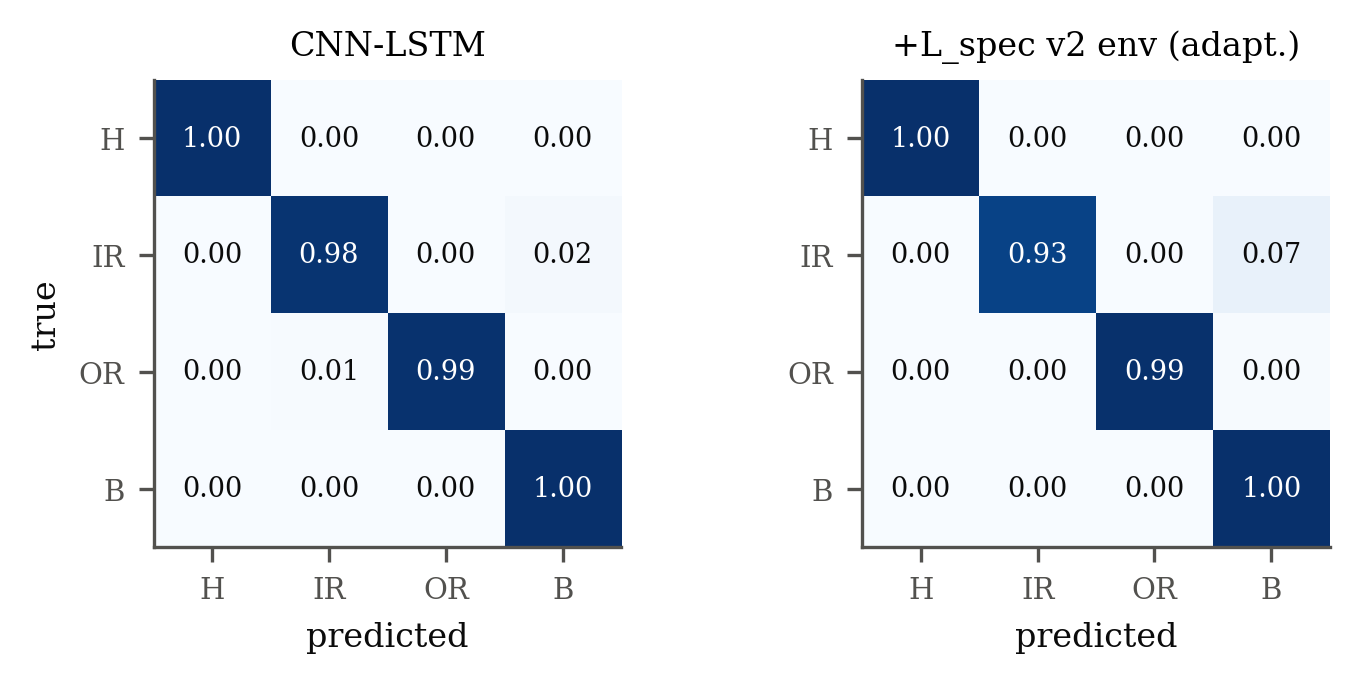
\includegraphics[width=\columnwidth]{fig_confusion_real.png}
\caption{Row-normalised confusion matrices on the held-out 3\,hp recordings,
summed over five seeds (H: healthy, IR: inner race, OR: outer race, B: ball).}
\label{fig:cm}
\end{figure}

\subsection{Fixed versus adaptive weighting}
Table~\ref{tab:weighting} compares fixed weights with the adaptive rule for the
envelope prior. Accuracy decreases monotonically as the fixed weight grows:
99.4\% at $\lambda=0.1$, 99.1\% at 0.5 and 98.4\% at 1.0. The adaptive rule
settles at a mean $\bar\lambda=0.91$ and behaves like a large fixed weight
(97.6\%), with the largest spread across seeds. None of these differences from
the baseline is significant. The data therefore do \emph{not} support the
claim that adaptive balancing helps. The best setting is the smallest weight,
i.e.\ the one closest to switching the prior off.

% --- generated by scripts/make_review03_tables.py (tables/tab_weighting.tex) ---
\begin{table}[t]
\caption{Fixed vs.\ adaptive weighting of $L_{\mathrm{spec}}^{\mathrm{v2}}$ (envelope), CWRU 0/1/2$\to$3\,hp (measured, 5 seeds).}
\label{tab:weighting}
\centering
\footnotesize
\begin{adjustbox}{max width=\columnwidth}
\begin{tabular}{lccc}
\toprule
Model & Test acc.\ (\%) & Mean $\lambda$ & $\Delta$ ($p$) \\
\midrule
CNN--LSTM ($\lambda=0$) & 99.3\,$\pm$\,1.0 & 0 & -- \\
+ $L_{\mathrm{spec}}^{\mathrm{v2}}$ envelope, fixed $\lambda=0.1$ & 99.4\,$\pm$\,0.4 & 0.1 & +0.17 (0.676) \\
+ $L_{\mathrm{spec}}^{\mathrm{v2}}$ envelope, fixed $\lambda=0.5$ & 99.1\,$\pm$\,0.7 & 0.5 & -0.17 (0.693) \\
+ $L_{\mathrm{spec}}^{\mathrm{v2}}$ envelope, fixed $\lambda=1.0$ & 98.4\,$\pm$\,2.1 & 1 & -0.90 (0.168) \\
+ $L_{\mathrm{spec}}^{\mathrm{v2}}$ envelope, adaptive & 97.6\,$\pm$\,3.5 & 0.905 & -1.63 (0.259) \\
\bottomrule
\end{tabular}
\end{adjustbox}
\end{table}


\subsection{Single-source extrapolation (0$\to$3\,hp)}
Training on 0\,hp alone makes the task genuinely hard
(Table~\ref{tab:single}). The CNN--LSTM falls to 87.1\,$\pm$\,6.2\%, mostly
because inner-race windows are confused with outer-race and ball faults. The
prior does not change this significantly:
\begin{itemize}
\item raw spectrum: 88.2\,$\pm$\,4.4\%, $\Delta=+1.1$, $p=0.62$;
\item envelope: 86.9\,$\pm$\,4.8\%, $\Delta=-0.2$, $p=0.83$;
\item transductive variant: 83.3\,$\pm$\,6.5\%, with macro-F1 dropping to
73.8\%. In some seeds it labels the healthy 3\,hp recording as outer-race.
\end{itemize}

% --- generated by scripts/make_review03_tables.py (tables/tab_single.tex) ---
\begin{table}[t]
\caption{Single-source extrapolation on CWRU: train on 0\,hp only, test on 3\,hp (measured, 5 seeds).}
\label{tab:single}
\centering
\footnotesize
\begin{adjustbox}{max width=\columnwidth}
\begin{tabular}{lccc}
\toprule
Model & Test acc.\ (\%) & Macro-F1 (\%) & $\Delta$ ($p$) \\
\midrule
CNN--LSTM ($\lambda=0$) & 87.1\,$\pm$\,6.2 & 88.2\,$\pm$\,6.0 & -- \\
+ $L_{\mathrm{spec}}^{\mathrm{v2}}$ raw spectrum, adaptive & 88.2\,$\pm$\,4.4 & 89.5\,$\pm$\,4.5 & +1.05 (0.621) \\
+ $L_{\mathrm{spec}}^{\mathrm{v2}}$ envelope, adaptive & 86.9\,$\pm$\,4.8 & 88.1\,$\pm$\,4.9 & -0.24 (0.825) \\
+ $L_{\mathrm{spec}}^{\mathrm{v2}}$ envelope + unlabelled target$^{\dagger}$ & 83.3\,$\pm$\,6.5 & 73.8\,$\pm$\,19.2 & -3.79 (0.369) \\
\bottomrule
\end{tabular}
\end{adjustbox}
\end{table}


\subsection{Robustness to noise and speed change}
Table~\ref{tab:robust} and Fig.~\ref{fig:robust} evaluate the trained
cross-load models on corrupted 3\,hp recordings:
\begin{itemize}
\item \emph{Noise.} All CNN--LSTM variants degrade similarly: about 97\% at
5\,dB, 76--84\% at 0\,dB and 44--51\% at $-5$\,dB. At 0\,dB the raw-spectrum
prior is significantly worse than the baseline ($-8.3$ points, $p=0.03$). No
variant is significantly better at any noise level. The random forest
collapses earlier (55\% at 0\,dB), and the Transformer is the least robust
model.
\item \emph{Speed.} Under a $\times1.05$ time-warp the envelope prior and v1
reach 99.4\% and 99.3\% versus 96.0\% for the baseline ($+3.4$ points,
$p=0.08$ and $p=0.07$). Under $\times0.95$ all CNN--LSTM variants fall to
78--83\% with wide intervals.
\end{itemize}
The speed trend is the only hint of a benefit in this study. It is not
significant at five seeds, and the speed change is emulated.

% --- generated by scripts/make_review03_tables.py (tables/tab_robust.tex) ---
\begin{table*}[t]
\caption{Robustness on the held-out 3\,hp recordings: additive white noise at the given SNR and emulated speed change (time-warp). Accuracy, \% (measured, 5 seeds; models trained on clean 0--2\,hp data only).}
\label{tab:robust}
\centering
\footnotesize
\begin{adjustbox}{max width=\textwidth}
\begin{tabular}{lccccccc}
\toprule
Model & 10 dB & 5 dB & 0 dB & -5 dB & $\times0.95$ & $\times1.05$ & $\pm5\%$ \\
\midrule
Random forest (12 features) & 94.0\,$\pm$\,0.4 & 82.5\,$\pm$\,5.4 & 54.9\,$\pm$\,7.1 & 58.3\,$\pm$\,4.1 & 61.6\,$\pm$\,0.5 & 70.3\,$\pm$\,0.7 & 62.8\,$\pm$\,0.3 \\
CNN--LSTM ($\lambda=0$) & 99.4\,$\pm$\,0.7 & 97.5\,$\pm$\,1.4 & 83.9\,$\pm$\,10.4 & 50.6\,$\pm$\,12.3 & 78.8\,$\pm$\,15.8 & 96.0\,$\pm$\,4.1 & 94.1\,$\pm$\,4.6 \\
+ $L_{\mathrm{spec}}^{\mathrm{v2}}$ raw spectrum, adaptive & 99.0\,$\pm$\,0.8 & 96.1\,$\pm$\,3.2 & 75.6\,$\pm$\,9.9 & 44.1\,$\pm$\,4.7 & 78.4\,$\pm$\,5.1 & 95.0\,$\pm$\,8.7 & 93.3\,$\pm$\,2.2 \\
+ $L_{\mathrm{spec}}^{\mathrm{v2}}$ envelope, adaptive & 98.2\,$\pm$\,3.6 & 96.9\,$\pm$\,2.3 & 77.1\,$\pm$\,16.3 & 48.7\,$\pm$\,7.4 & 81.1\,$\pm$\,5.3 & 99.4\,$\pm$\,0.3 & 94.5\,$\pm$\,2.8 \\
+ $L_{\mathrm{spec}}^{\mathrm{v2}}$ envelope + unlabelled target$^{\dagger}$ & 89.7\,$\pm$\,0.5 & 89.4\,$\pm$\,2.9 & 80.2\,$\pm$\,15.5 & 46.5\,$\pm$\,7.2 & 72.8\,$\pm$\,13.0 & 92.6\,$\pm$\,3.5 & 87.0\,$\pm$\,2.7 \\
\bottomrule
\end{tabular}
\end{adjustbox}
\end{table*}


\begin{figure*}[t]
\centering
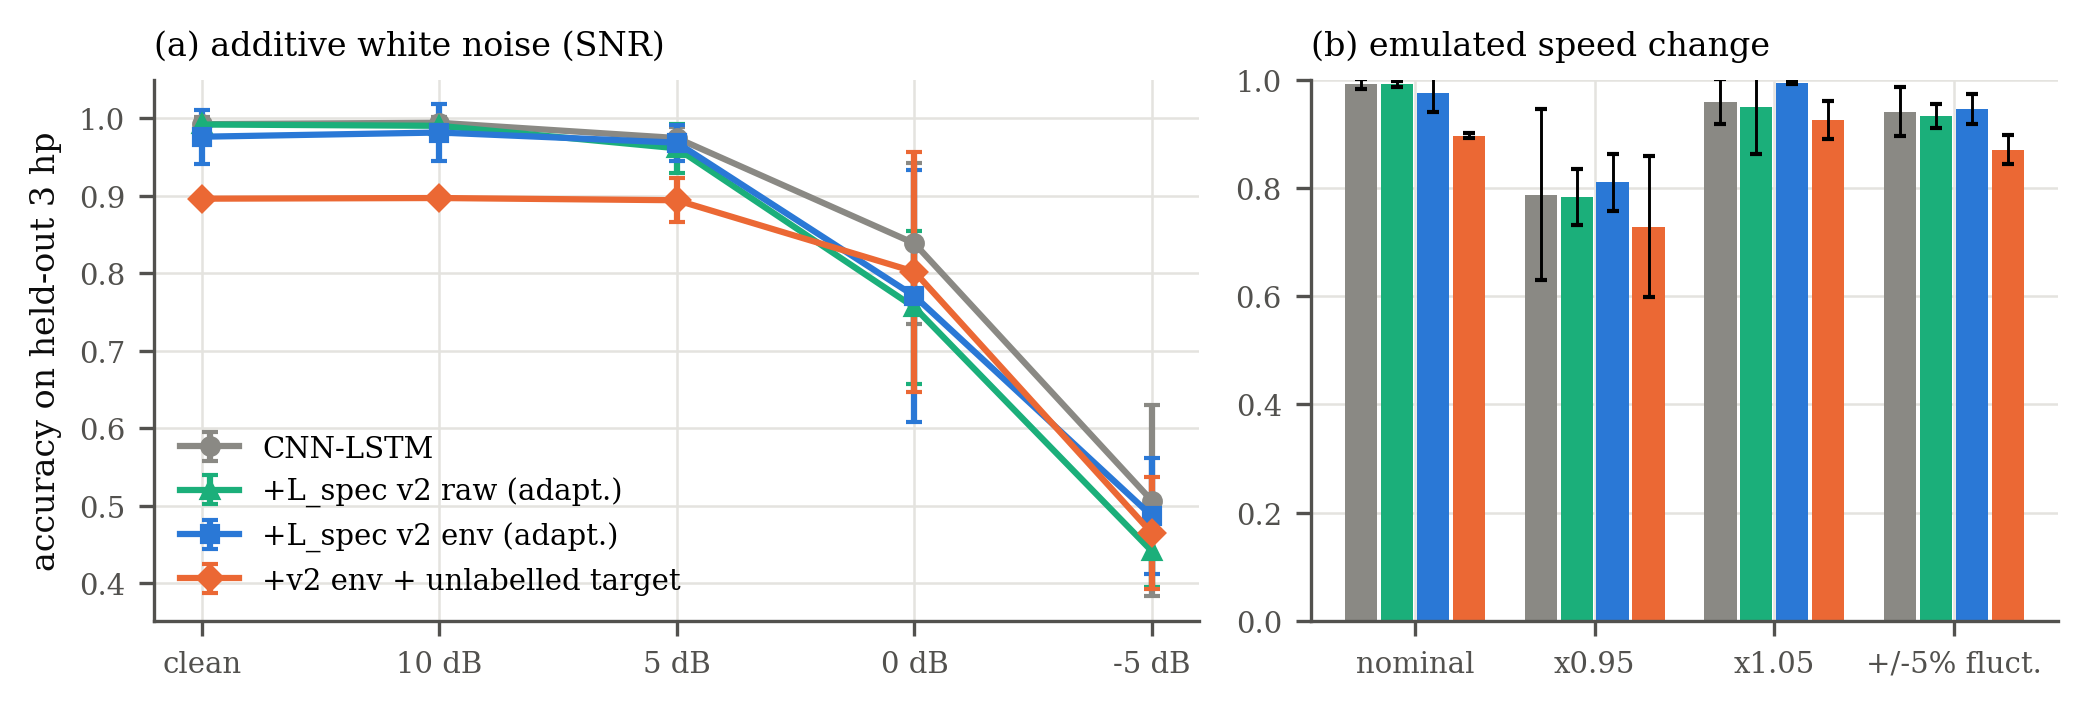
\includegraphics[width=0.85\textwidth]{fig_robustness.png}
\caption{Accuracy of the cross-load models (trained on clean 0--2\,hp data) on
corrupted 3\,hp recordings; mean and 95\% CI over five seeds. The legend in (a)
also applies to (b).}
\label{fig:robust}
\end{figure*}

\subsection{Second dataset: MFPT (preliminary)}
The MFPT runs were stopped before completion: three seeds for the CNN, the
CNN--LSTM and the raw-spectrum prior, and two seeds for the envelope variants,
so Table~\ref{tab:mfpt} is preliminary. We deliberately do \emph{not} transfer a
trained model from CWRU to MFPT. The two rigs differ in accelerometer placement
and sampling rate, in bearing geometry, in the fault types present, and in class
balance, so a CWRU$\to$MFPT score would confound sensor-configuration,
operating-condition, fault-type and class-distribution effects and could not be
attributed to the prior. MFPT is instead an \emph{independent} replication of
the within-dataset load-shift protocol, with its own leakage-controlled splits,
so each dataset is judged only against itself. The load shift on MFPT defeats every
supervised model, at 29--39\% accuracy, near chance for three classes. The
confusion matrices show why. Healthy data exist only at 270\,lbs, so the
models associate the high-load signature with ``healthy'' and label most
270--300\,lbs outer-race windows as healthy. This is a confound of
load and class in the MFPT design, not a property of the method. The
supervised envelope prior does not remove it (33\%). The transductive envelope
variant classified all test windows correctly in both completed seeds. This is
the only setting in which the prior had a large effect. But it rests on two
seeds and on access to unlabelled target data, and it reverses the CWRU
finding. The sensitivity analysis explains the reversal
(Table~\ref{tab:sens}). On MFPT the envelope evidence identifies the fault type
of 100\% of the training and test windows (raw spectrum: 73--79\%), so the
unlabelled target windows receive correct pseudo-labels and break the
load/class confound. On CWRU the same evidence is right for only about 64\%,
and applying it to unlabelled windows hurts. The MFPT accuracies themselves
rest on two to three seeds and should be read as preliminary; the evidence
accuracy, which needs no training, is a complete measurement.

% --- generated by scripts/make_review03_tables.py (tables/tab_mfpt.tex) ---
\begin{table}[t]
\caption{Second bearing dataset (MFPT, \emph{preliminary}): faults trained at 0--150\,lbs, tested at 270--300\,lbs. Measured; $n$ = number of completed seeds (CI from $n$ seeds; no CI is meaningful for $n=2$).}
\label{tab:mfpt}
\centering
\footnotesize
\begin{adjustbox}{max width=\columnwidth}
\begin{tabular}{lccc}
\toprule
Model & $n$ & Test acc.\ (\%) & Macro-F1 (\%) \\
\midrule
Random forest (12 features) & 5 & 29.9\,$\pm$\,0.0 & 29.8\,$\pm$\,0.0 \\
SVM-RBF (12 features) & 5 & 29.3\,$\pm$\,0.0 & 29.0\,$\pm$\,0.0 \\
CNN & 3 & 30.2\,$\pm$\,2.0 & 32.4\,$\pm$\,8.6 \\
CNN--LSTM ($\lambda=0$) & 3 & 39.2\,$\pm$\,21.5 & 41.2\,$\pm$\,26.5 \\
\midrule
+ $L_{\mathrm{spec}}^{\mathrm{v2}}$ raw spectrum, adaptive & 3 & 34.5\,$\pm$\,16.9 & 36.2\,$\pm$\,12.2 \\
+ $L_{\mathrm{spec}}^{\mathrm{v2}}$ envelope, adaptive & 2 & 33.3\,$\pm$\,17.3 & 37.1\,$\pm$\,59.0 \\
+ $L_{\mathrm{spec}}^{\mathrm{v2}}$ envelope, fixed $\lambda=0.5$ & 2 & 32.7\,$\pm$\,17.3 & 36.3\,$\pm$\,60.4 \\
+ $L_{\mathrm{spec}}^{\mathrm{v2}}$ envelope + unlabelled target$^{\dagger}$ & 2 & 100.0\,$\pm$\,0.0 & 100.0\,$\pm$\,0.0 \\
\bottomrule
\end{tabular}
\end{adjustbox}
\par\vspace{2pt}\parbox{\columnwidth}{\scriptsize $^{\dagger}$Transductive (unlabelled target inputs used in training).}
\end{table}


\subsection{Sensitivity to band width and harmonics}
Table~\ref{tab:sens} reports the evidence accuracy over the full grid. On the
held-out 3\,hp CWRU windows the envelope evidence lies between 51.0\% and
67.2\%. It is best and most stable for narrow bands ($\sigma\le5$\,Hz: 62.6--67.2\%
for all $H$) and degrades as the bands widen. Wide bands do not add
information; they only move the errors between classes. At $\sigma=20$\,Hz,
$H=3$ ball recall rises to 91.5\% while outer-race recall falls to 39.5\%.
Our pre-set default ($\sigma=5$\,Hz, $H=3$, 64.1\%) is within 3.1 points of the
best setting. The raw spectrum stays at or near chance level (29.0--45.1\%) for
every setting, which confirms that the defect frequencies must be demodulated
before they can serve as a prior.

The physical prior is therefore robust to its hyper-parameters, in the sense
that no setting changes its quality materially. For the same reason, no
setting can make it reliable on CWRU: about one fault window in three always
receives a wrong spectral pseudo-label. We did not repeat the end-to-end
training for every grid cell. Given the 3-point range of evidence accuracy, and
given that the cross-load results already show no benefit at the best-informed
setting, a different $\sigma$ or $H$ is unlikely to change the conclusions.

\begin{table}[t]
\caption{Training-free sensitivity of the spectral prior: evidence accuracy
(\%) of the fault type on faulty windows (measured). Top: CWRU held-out
3\,hp recordings, envelope spectrum; default setting in bold.}
\label{tab:sens}
\centering
\footnotesize
\begin{adjustbox}{max width=\columnwidth}
\begin{tabular}{lccc}
\toprule
Envelope, CWRU 3\,hp & $H=1$ & $H=3$ & $H=5$ \\
\midrule
$\sigma=2$\,Hz  & 66.3 & 67.2 & 66.7 \\
$\sigma=5$\,Hz  & 64.6 & \textbf{64.1} & 62.6 \\
$\sigma=10$\,Hz & 58.9 & 59.8 & 59.6 \\
$\sigma=20$\,Hz & 51.0 & 61.8 & 54.9 \\
\midrule
Raw spectrum, CWRU 3\,hp (all 12 settings) & \multicolumn{3}{c}{29.0--45.1 (33.4 for $H\le3$)} \\
\midrule
MFPT test ($\sigma=5$, $H=3$): envelope & \multicolumn{3}{c}{100.0} \\
MFPT test ($\sigma=5$, $H=3$): raw & \multicolumn{3}{c}{79.0} \\
\bottomrule
\end{tabular}
\end{adjustbox}
\end{table}

%=====================================================================
\section{Ablation Studies}
\label{sec:ablation}
%=====================================================================
To isolate the contribution of each design choice, we ablate the full model
one component at a time on the main CWRU 0/1/2$\to$3\,hp protocol. The full
model is the CNN--LSTM with $\Lspec^{\mathrm{v2}}$ on the envelope spectrum,
adaptive weighting, $\sigma=5$\,Hz and $H=3$. Each ablation changes exactly
one component and keeps everything else fixed: network, inputs, splits,
optimiser, epochs, early stopping and seeds. Table~\ref{tab:ablation} reports
the paired per-seed difference from the full model; positive values mean the
ablated variant is better. Ablations of the physics settings that need no
training are measured through the evidence accuracy of the prior.

\begin{table}[t]
\caption{Ablation study on CWRU 0/1/2$\to$3\,hp (measured, 5 seeds). Full
model: CNN--LSTM + $\Lspec^{\mathrm{v2}}$, envelope, adaptive, $\sigma=5$\,Hz,
$H=3$. $\Delta$: paired difference vs.\ the full model (percentage points,
$\pm$95\% CI), paired $t$-test $p$.}
\label{tab:ablation}
\centering
\footnotesize
\begin{adjustbox}{max width=\columnwidth}
\begin{tabular}{llccc}
\toprule
ID & Ablated component & Acc.\ (\%) & $\Delta$ & $p$ \\
\midrule
-- & Full model & 97.6 & -- & -- \\
\midrule
A1 & Remove physics term ($\lambda=0$) & 99.3 & $+1.63\pm3.44$ & 0.26 \\
A2 & v2 loss $\to$ v1 loss (64-bin STFT) & 99.2 & $+1.58\pm3.02$ & 0.22 \\
A3 & Envelope $\to$ raw spectrum & 99.2 & $+1.58\pm3.64$ & 0.30 \\
A4a & Adaptive $\to$ fixed $\lambda=0.1$ & 99.4 & $+1.80\pm3.21$ & 0.19 \\
A4b & Adaptive $\to$ fixed $\lambda=0.5$ & 99.1 & $+1.46\pm2.77$ & 0.22 \\
A4c & Adaptive $\to$ fixed $\lambda=1.0$ & 98.4 & $+0.73\pm4.52$ & 0.68 \\
A5 & Add unlabelled target windows$^{\dagger}$ & 89.6 & $-8.00\pm3.18$ & 0.002 \\
\midrule
\multicolumn{5}{l}{\emph{Training-data ablation: train on 0\,hp only (0$\to$3\,hp)}} \\
A6 & Full model & 86.9 & -- & -- \\
A6a & \quad remove physics term & 87.1 & $+0.24\pm2.80$ & 0.83 \\
A6b & \quad envelope $\to$ raw & 88.2 & $+1.29\pm6.20$ & 0.59 \\
A6c & \quad add unlabelled target$^{\dagger}$ & 83.3 & $-3.55\pm7.74$ & 0.27 \\
\midrule
\multicolumn{5}{l}{\emph{Training-free ablations: evidence accuracy of the prior (\%)}} \\
A7 & Spectral view: STFT-64 / raw / envelope & \multicolumn{3}{c}{32.3 / 33.3 / 66.4} \\
A8 & Band width $\sigma$ (2--20\,Hz), $H=3$ & \multicolumn{3}{c}{67.2 / 64.1 / 59.8 / 61.8} \\
A9 & Harmonics $H$ (1 / 3 / 5), $\sigma=5$\,Hz & \multicolumn{3}{c}{64.6 / 64.1 / 62.6} \\
\bottomrule
\end{tabular}
\end{adjustbox}
\par\vspace{2pt}\parbox{\columnwidth}{\scriptsize $^{\dagger}$Transductive: uses
the unlabelled target-load inputs, never their labels. A7 on 0--2\,hp training
windows; A8--A9 on the held-out 3\,hp windows.}
\end{table}

\textbf{What the ablations show.}
\begin{itemize}
\item \emph{Removing the physics term (A1)} does not hurt; it gives the
numerically best accuracy among supervised variants, so the term contributes
no measurable gain.
\item \emph{The corrected loss (A2), the envelope view (A3) and adaptive
weighting (A4a--c)} each perform no better than their simpler alternative.
Every swap moves accuracy toward the no-physics baseline, and the smallest
fixed weight comes closest to it. None of A1--A4 is significant at five seeds,
so the components are statistically neutral on CWRU.
\item \emph{The transductive variant (A5)} is the only significant ablation,
and it is harmful ($-8.0$ points, $p=0.002$).
\item \emph{With less training diversity (A6)} the same pattern holds.
\item \emph{The training-free ablations (A7--A9)} explain why. The prior is
only informative after envelope demodulation (A7). Its quality depends little
on band width and harmonic count within the narrow-band range (A8--A9).
It stays near 64--67\%, which is too unreliable to improve a classifier that
is already at 99\%.
\end{itemize}

%=====================================================================
\section{Discussion}
\label{sec:discussion}
%=====================================================================
Taken together, the measurements answer the questions posed in the review:
\begin{enumerate}
\item On the original CWRU recordings, the 0/1/2$\to$3\,hp shift costs the
plain CNN--LSTM less than one point. There is little degradation for a prior
to repair, and the earlier expectation of a large drop was not borne out once
real data were used.
\item With the network fixed, adding the spectral prior does not improve accuracy
in any CWRU protocol. The ranking follows the informativeness of the evidence,
inverted: the uninformative v1 and raw-spectrum priors are harmless, while the
informative but imperfect envelope prior injects wrong pseudo-labels and hurts.
This is the behaviour the reviewer anticipated in point~2. A prior that was
always right on constructed data is right only about two times in three on real
envelope spectra.
\item Adaptive weighting is not better than a small fixed weight.
\item Fixing the loss (v2) was necessary for the term to have any effect at all,
but a correct loss does not make the prior useful.
\item The value of the prior is set by the reliability of its spectral
evidence, not by its weighting or band settings. Evidence accuracy varies by
only about 3 points over the narrow-band settings. It is 64\% on CWRU, where the
prior does not help, and 100\% on MFPT, where the transductive variant recovers
from a failure of all supervised models.
\end{enumerate}
The contribution of this paper is therefore an evaluated negative result and a
corrected, tested formulation, not an accuracy improvement.

\section{Limitations and Threats to Validity}
\begin{itemize}
\item \emph{Splits.} CWRU has one recording per class, severity and load, so
the in-distribution protocol splits in time rather than by recording, and the
cross-load test set has ten recordings. Per-recording effects (e.g.\ one
inner-race record) can dominate the variance.
\item \emph{Seeds.} Five seeds detect differences of roughly one to two points
on CWRU; smaller effects cannot be excluded. MFPT accuracies rest on 2--3
seeds. The band-width/harmonic sensitivity is measured on the evidence accuracy
of the prior, not by retraining the classifier for every grid cell.
\item \emph{Speed.} Speed variation is emulated by time-warping, which also
shifts resonances. No genuinely variable-speed data were used. The prior also
presumes a known shaft speed: each mask is centred at $h\,r_c f_r$, so an error
in the estimated $f_r$ translates the mask off the true defect band and degrades
the evidence in proportion to the error. The prior is thus at most as reliable
as the speed estimate, and under inaccurately known or continuously varying
speed its spectral evidence---already the limiting factor on CWRU---can only
deteriorate.
\item \emph{Physics.} The prior is kinematic. Slip, load-zone modulation and
transmission effects are not modelled, and the envelope band (1--5.5\,kHz) is
fixed rather than selected per record (e.g.\ by spectral kurtosis).
\item \emph{Fixed choices.} All default settings ($\sigma=5$\,Hz, $H=3$,
$\rho=0.25$) were fixed in advance and not tuned on test data. This avoids
optimistic bias but means a better-tuned prior cannot be ruled out.
\end{itemize}

\section{Conclusion and Future Work}
We derived CWRU-PG, a physics-annotated, leakage-free dataset from the
original CWRU recordings, and used it to revise and ablate a
characteristic-frequency spectral prior for bearing diagnosis. We
evaluated it on the original CWRU recordings and on MFPT, with splits formed
before windowing, five seeds on CWRU and paired tests.

The original formulation was found to be defective. It is uninformative at its
input resolution, its gradient leaks into the healthy class, and its mixture
normalisation couples the gradient to mask mass. We derived and tested a
corrected version.

On real data, neither version improved cross-load accuracy over the identical
network without physics. The envelope-based prior and its transductive variant
reduced accuracy, because envelope evidence identifies the fault type for only
about two-thirds of the windows. The method is a physics-guided spectral prior,
not a PINN, and its value is limited by the reliability of that evidence.
The sensitivity analysis makes this concrete. No band-width or harmonic
setting lifts the evidence above 67\% on CWRU, whereas on MFPT it is 100\%
correct, and only there does the prior (applied to unlabelled target windows)
help.

Future work:
\begin{enumerate}
\item weight the prior by its own confidence, e.g.\ apply it only where the
evidence margin exceeds the 0.49 reliability limit of Table~\ref{tab:limits};
\item complete the MFPT runs to five seeds, retrain the classifier across the
sensitivity grid, and add a dataset with healthy data at several loads
(e.g.\ Paderborn);
\item test on genuinely variable-speed recordings;
\item replace the kinematic prior with a model-based residual, e.g.\ of the
McFadden--Smith impact model.
\end{enumerate}

%=====================================================================
\section{Reproducibility}
\label{sec:repro}
%=====================================================================
The submission archive includes the complete code, and its core is listed in
Appendix~\ref{app:code}. From the repository root,
after placing the 40 CWRU files in \texttt{data/raw/cwru/} and the MFPT files in
\texttt{data/raw/mfpt/}:
\begin{itemize}
\item \texttt{python scripts/run\_review03.py --exp all} trains and evaluates
every configuration and seed, caching one JSON file per run under
\texttt{outputs/review03/runs/};
\item \texttt{python scripts/make\_review03\_tables.py} and
\texttt{scripts/make\_review03\_figs.py} regenerate the result tables and figures from those files;
\item \texttt{python scripts/build\_derived\_dataset.py} generates CWRU-PG
(about 100\,MB, under a minute on a laptop CPU);
\item \texttt{python scripts/physics\_residuals.py} computes the residuals of
Table~\ref{tab:residuals};
\item \texttt{python scripts/constraint\_limits.py} computes the constraint
values and limits of Table~\ref{tab:limits} from CWRU-PG;
\item \texttt{python scripts/evidence\_sensitivity.py} computes the
training-free sensitivity of Table~\ref{tab:sens} in seconds;
\item \texttt{pytest tests/} runs the unit tests, including the leakage check
and the gradient properties of Eq.~\eqref{eq:v2}.
\end{itemize}
The loaders, protocols and losses are in \texttt{src/review03/}; the core of
the implementation is reproduced in Appendix~\ref{app:code}.

%=====================================================================
% Listings sit inside the normal IEEE columns; every code line is
% at most 58 characters so nothing wraps.
\appendices
\section{Core Training and Evaluation Code}
\label{app:code}
%=====================================================================
Listings~\ref{lst:split}--\ref{lst:stats} give the essential parts of the
implementation used for all results (Python 3.9, PyTorch 2.8, SciPy 1.13),
shortened only by removing logging and argument parsing: the split before
windowing with its leakage check (Listing~\ref{lst:split}), the spectral views
(Listing~\ref{lst:spec}), the revised term $\Lspec^{\mathrm{v2}}$
(Listing~\ref{lst:loss}), the shared training loop (Listing~\ref{lst:train}) and
the statistics (Listing~\ref{lst:stats}).

\begin{lstlisting}[caption={Split before windowing and leakage check.},label={lst:split}]
def time_blocks(rec, fracs, guard):
    """Cut one recording into consecutive
    blocks (e.g. 70/15/15) with guard gaps."""
    n = len(rec.signal)
    usable = n - guard * (len(fracs) - 1)
    segs, pos = [], 0
    for i, (name, frac) in enumerate(fracs):
        last = i == len(fracs) - 1
        size = n - pos if last else \
            int(round(usable * frac))
        stop = min(n, pos + size)
        segs.append(Segment(rec, pos, stop, name))
        pos += size + guard
    return segs

def cwru_protocol(recs, regime, win=2048):
    segs = []
    for r in recs:
        if regime == "in_distribution":
            segs += time_blocks(r, [("train", .70),
                ("val", .15), ("test", .15)], win)
        elif int(r.load) == 3:   # cross-load test
            segs.append(
                Segment(r, 0, len(r.signal), "test"))
        else:
            segs += time_blocks(r, [("train", .85),
                ("val", .15)], win)
    return segs

def window_segment(seg, win=2048, hop=1024):
    """Windows are cut strictly inside a segment."""
    starts = np.arange(seg.start,
                       seg.stop - win + 1, hop)
    idx = starts[:, None] + np.arange(win)[None]
    return seg.rec.signal[idx], starts

def assert_no_overlap(index, win):
    """Fail if windows of two splits share
    a sample of the same recording."""
    names = list(index)
    for i, a in enumerate(names):
        for b in names[i + 1:]:
            A, B = index[a], index[b]
            for rec in np.intersect1d(A["rec"],
                                      B["rec"]):
                sa = np.sort(A["start"][A["rec"] == rec])
                sb = np.sort(B["start"][B["rec"] == rec])
                pos = np.searchsorted(sb, sa)
                for k, s in zip(pos, sa):
                    for j in (k - 1, k):
                        if 0 <= j < len(sb) and \
                           abs(sb[j] - s) < win:
                            raise AssertionError(
                                "window leakage")
\end{lstlisting}

\begin{lstlisting}[caption={High-resolution raw and squared-envelope spectra.},label={lst:spec}]
def spectral_views(w, fs, f_max=1000.0,
                   band=(1000.0, 5500.0)):
    n = w.shape[1]
    hann = np.hanning(n)[None]
    freqs = np.fft.rfftfreq(n, 1.0 / fs)  # 5.9 Hz
    keep = freqs <= f_max
    x = w - w.mean(axis=1, keepdims=True)
    raw = np.abs(np.fft.rfft(x * hann)) ** 2
    hi = min(band[1], 0.45 * fs)
    sos = signal.butter(4, [band[0], hi],
                        btype="bandpass", fs=fs,
                        output="sos")
    xb = signal.sosfiltfilt(sos, x, axis=1)
    env = np.abs(signal.hilbert(xb)) ** 2
    env -= env.mean(axis=1, keepdims=True)
    envs = np.abs(np.fft.rfft(env * hann)) ** 2
    return raw[:, keep], envs[:, keep], freqs[keep]
\end{lstlisting}

\begin{lstlisting}[caption={Per-window masks and the revised term $L_{\mathrm{spec}}^{\mathrm{v2}}$ (Eq.~\eqref{eq:v2}).},label={lst:loss}]
def build_masks(freqs, ratios, shaft_hz,
                H=3, sigma=5.0):
    """(B, C, F) Gaussian masks at h*r_c*f_r,
    unit sum; zero row for healthy (None)."""
    f = torch.as_tensor(freqs, dtype=torch.float32)
    B, C = shaft_hz.shape[0], len(ratios)
    masks = torch.zeros(B, C, f.numel())
    for c, r in enumerate(ratios):
        if r is None:
            continue
        f0 = (r * shaft_hz)[:, None]
        m = 0
        for h in range(1, H + 1):
            on = (h * f0 <= f.max()).float()
            d = (f[None] - h * f0) / sigma
            m = m + on * torch.exp(-0.5 * d ** 2)
        masks[:, c] = m / (m.sum(1, keepdim=True)
                           + 1e-12)
    return masks

def spectral_loss_v2(spec, logits, masks, valid,
                     eps=1e-12):
    s = spec / (spec.sum(1, keepdim=True) + eps)
    e = torch.einsum("bf,bcf->bc", s, masks)
    e = e * valid[None]
    ebar = e / (e.amax(1, keepdim=True) + eps)
    ebar = ebar.detach()
    p = torch.softmax(logits, 1)
    # stop-gradient window weight
    w = (p * valid[None]).sum(1).detach()
    # softmax over fault logits only
    z = logits.masked_fill(valid[None] == 0,
                           float("-inf"))
    pt = torch.softmax(z, 1)
    align = (pt * ebar).sum(1)
    return (w * (1 - align)).sum() / (w.sum() + eps)
\end{lstlisting}

\begin{lstlisting}[caption={Training loop shared by all neural models (baseline: \texttt{phys=None}).},label={lst:train}]
def train(model, tr, va, phys, ratios, freqs,
          seed, epochs=30, bs=64, lr=1e-3,
          patience=8, rho=0.25, alpha=0.12):
    torch.manual_seed(seed)
    C = len(ratios)
    cnt = np.bincount(tr.y, minlength=C)
    cw = torch.tensor(cnt.sum() / (C * cnt),
                      dtype=torch.float32)
    opt = torch.optim.Adam(model.parameters(), lr)
    sched = torch.optim.lr_scheduler \
        .CosineAnnealingLR(opt, epochs)
    valid = torch.tensor(
        [0. if r is None else 1. for r in ratios])
    masks = (build_masks(freqs, ratios, tr.shaft_hz)
             if phys else None)
    lam = phys["lam"] if phys else 0.0
    best, bad, state = 1e9, 0, None
    shared = list(model.backbone.parameters())
    for ep in range(epochs):
        model.train()
        perm = torch.randperm(len(tr.y))
        for idx in perm.split(bs):
            out = model(tr.x[idx], tr.feat[idx])
            logits = out["logits"]
            l_data = F.cross_entropy(
                logits, tr.y[idx], weight=cw)
            loss = l_data
            if phys:
                spec = tr.spec[phys["view"]][idx]
                l_spec = spectral_loss_v2(
                    spec, logits, masks[idx], valid)
                if phys["adaptive"]:
                    g_d = grad_norm(l_data, shared)
                    g_s = grad_norm(l_spec, shared)
                    tgt = rho * g_d / (g_s + 1e-8)
                    lam = (1 - alpha) * lam \
                        + alpha * tgt
                    lam = min(max(lam, 1e-3), 1e2)
                loss = l_data + lam * l_spec
            opt.zero_grad()
            loss.backward()
            torch.nn.utils.clip_grad_norm_(
                model.parameters(), 5.0)
            opt.step()
        sched.step()
        vl = val_loss(model, va, cw)  # early stop
        if vl < best - 1e-5:
            best, bad = vl, 0
            state = copy.deepcopy(model.state_dict())
        else:
            bad += 1
            if bad >= patience:
                break
    model.load_state_dict(state)
    return model

def grad_norm(loss, params):
    g = torch.autograd.grad(loss, params,
                            retain_graph=True,
                            allow_unused=True)
    sq = sum(float(x.pow(2).sum())
             for x in g if x is not None)
    return sq ** 0.5
\end{lstlisting}

\begin{lstlisting}[caption={Statistics: 95\% CI and paired test against the baseline.},label={lst:stats}]
def ci95(v):
    v = np.asarray(v, float)
    t = stats.t.ppf(0.975, len(v) - 1)
    return v.mean(), t * v.std(ddof=1) / len(v) ** .5

def paired(acc_model, acc_base):  # seeds 0..4
    d = np.subtract(acc_model, acc_base)
    p = None
    if d.std() > 0:
        p = stats.ttest_rel(acc_model,
                            acc_base).pvalue
    return d.mean(), ci95(d)[1], p
\end{lstlisting}

%=====================================================================
\begin{thebibliography}{00}
\bibitem{raissi2019} M. Raissi, P. Perdikaris, and G. E. Karniadakis,
``Physics-informed neural networks: A deep learning framework for solving
forward and inverse problems involving nonlinear partial differential
equations,'' \textit{J. Comput. Phys.}, vol. 378, pp. 686--707, 2019.
\bibitem{mcfadden1984} P. D. McFadden and J. D. Smith, ``Model for the vibration
produced by a single point defect in a rolling element bearing,'' \textit{J.
Sound Vib.}, vol. 96, no. 1, pp. 69--82, 1984.
\bibitem{randall2011} R. B. Randall and J. Antoni, ``Rolling element bearing
diagnostics---A tutorial,'' \textit{Mech. Syst. Signal Process.}, vol. 25, no.
2, pp. 485--520, 2011.
\bibitem{smith2015} W. A. Smith and R. B. Randall, ``Rolling element bearing
diagnostics using the Case Western Reserve University data: A benchmark study,''
\textit{Mech. Syst. Signal Process.}, vol. 64--65, pp. 100--131, 2015.
\bibitem{zhang2017} W. Zhang, G. Peng, C. Li, Y. Chen, and Z. Zhang, ``A new
deep learning model for fault diagnosis with good anti-noise and domain
adaptation ability on raw vibration signals,'' \textit{Sensors}, vol. 17, no. 2,
art. 425, 2017.
\bibitem{wen2018} L. Wen, X. Li, L. Gao, and Y. Zhang, ``A new convolutional
neural network-based data-driven fault diagnosis method,'' \textit{IEEE Trans.
Ind. Electron.}, vol. 65, no. 7, pp. 5990--5998, 2018.
\bibitem{lei2020} Y. Lei, B. Yang, X. Jiang, F. Jia, N. Li, and A. K. Nandi,
``Applications of machine learning to machine fault diagnosis: A review and
roadmap,'' \textit{Mech. Syst. Signal Process.}, vol. 138, art. 106587, 2020.
\bibitem{hoang2019} D. T. Hoang and H. J. Kang, ``A survey on deep learning based
bearing fault diagnosis,'' \textit{Neurocomputing}, vol. 335, pp. 327--335,
2019.
\bibitem{zhao2020} Z. Zhao, T. Li, J. Wu, C. Sun, S. Wang, R. Yan, and X. Chen,
``Deep learning algorithms for rotating machinery intelligent diagnosis: An
open source benchmark study,'' \textit{ISA Trans.}, vol. 107, pp. 224--255, 2020.
\bibitem{alam2025} S. Alam \textit{et al.}, ``Physics-informed multimodal bearing
fault classification under variable operating conditions using transfer
learning,'' \textit{arXiv preprint} arXiv:2508.07536, 2025.
\bibitem{costa2022} P. R. de Oliveira da Costa \textit{et al.}, ``T4PdM: A deep
neural network based on the Transformer architecture for fault diagnosis of
rotating machinery,'' \textit{arXiv preprint} arXiv:2204.03725, 2022.
\bibitem{mcclenny2023} L. McClenny and U. Braga-Neto, ``Self-adaptive
physics-informed neural networks,'' \textit{J. Comput. Phys.}, vol. 474, art.
111722, 2023.
\bibitem{wang2021} S. Wang, Y. Teng, and P. Perdikaris, ``Understanding and
mitigating gradient flow pathologies in physics-informed neural networks,''
\textit{SIAM J. Sci. Comput.}, vol. 43, no. 5, pp. A3055--A3081, 2021.
\bibitem{cwru} Case Western Reserve University Bearing Data Center, ``CWRU
bearing fault dataset,'' [Online]. Available:
https://engineering.case.edu/bearingdatacenter
\bibitem{mfpt} Society for Machinery Failure Prevention Technology, ``MFPT
bearing fault data sets,'' 2013.
\bibitem{jardine2006} A. K. S. Jardine, D. Lin, and D. Banjevic, ``A review on
machinery diagnostics and prognostics implementing condition-based
maintenance,'' \textit{Mech. Syst. Signal Process.}, vol. 20, no. 7, pp.
1483--1510, 2006.
\end{thebibliography}

\end{document}
